\documentclass{article}

% if you need to pass options to natbib, use, e.g.:
     \PassOptionsToPackage{numbers, sort&compress}{natbib}
% before loading neurips_2021

% ready for submission
\usepackage{neurips_2021}
\usepackage{comment}
% to compile a preprint version, e.g., for submission to arXiv, add add the
% [preprint] option:
%     \usepackage[preprint]{neurips_2021}

% to compile a camera-ready version, add the [final] option, e.g.:
%     \usepackage[final]{neurips_2021}

% to avoid loading the natbib package, add option nonatbib:
%    \usepackage[nonatbib]{neurips_2021}

\usepackage[utf8]{inputenc} % allow utf-8 input
\usepackage[T1]{fontenc}    % use 8-bit T1 fonts
\usepackage{hyperref}       % hyperlinks
\usepackage{url}            % simple URL typesetting
\usepackage{booktabs}       % professional-quality tables
\usepackage{amsfonts}       % blackboard math symbols
\usepackage{nicefrac}       % compact symbols for 1/2, etc.
\usepackage{microtype}      % microtypography
\usepackage{xcolor}         % colors
\usepackage{rotating}
\usepackage{multirow}
%\usepackage{natbib}
\usepackage{graphicx}
\usepackage{subcaption}
\usepackage{soul}
\usepackage{enumitem}
\usepackage{bm}
\usepackage{amsmath}
\usepackage{amssymb}
\newcommand{\jd}[1]{\textcolor{orange}{[DJ: #1]}}
\newcommand{\jdtext}[1]{\textcolor{red}{#1}}
\newcommand{\aq}[1]{\textcolor{purple}{[AQ: #1]}}
\newcommand{\drop}[1]{\begin{scriptsize}{\textcolor{green}{[#1]}}\end{scriptsize}}


%Includes "References" in the table of contents
\usepackage[nottoc]{tocbibind}

%Import the natbib package and sets a bibliography style
%\usepackage[round,numbers]{natbib}
%\bibliographystyle{ksfh_nat}
\bibliographystyle{plainnat}

\title{Object Representations Guided By Optical Flow}

% The \author macro works with any number of authors. There are two commands
% used to separate the names and addresses of multiple authors: \And and \AND.
%
% Using \And between authors leaves it to LaTeX to determine where to break the
% lines. Using \AND forces a line break at that point. So, if LaTeX puts 3 of 4
% authors names on the first line, and the last on the second line, try using
% \AND instead of \And before the third author name.

\author{%
  David S.~Hippocampus\thanks{Use footnote for providing further information
    about author (webpage, alternative address)---\emph{not} for acknowledging
    funding agencies.} \\
  Department of Computer Science\\
  Cranberry-Lemon University\\
  Pittsburgh, PA 15213 \\
  \texttt{hippo@cs.cranberry-lemon.edu} \\
  % examples of more authors
  % \And
  % Coauthor \\
  % Affiliation \\
  % Address \\
  % \texttt{email} \\
  % \AND
  % Coauthor \\
  % Affiliation \\
  % Address \\
  % \texttt{email} \\
  % \And
  % Coauthor \\
  % Affiliation \\
  % Address \\
  % \texttt{email} \\
  % \And
  % Coauthor \\
  % Affiliation \\
  % Address \\
  % \texttt{email} \\
}

\begin{document}

\maketitle

  % and use this signal through optical flow approaches to learn object-centric representations. 
  
  % and optical flow approaches extract such signals very effectively.
  
  %This often involves training structured object encoders through reconstruction or prediction objectives or contrastive losses.  
  %Learning object-centric representation directly from low-level perception data is an important step towards fully automated robotics control. Previous methods either rely on input action information or image reconstruction to provide inductive bias for learning object-centric representation. In contrast, we designed an optical-flow based object representation learning method. Specifically, we use object motion as supervision for learning object-centric representations from perception data of unlabeled control sequences. Without any action label, our method achieves the same-level of performances comparing to methods that requires those labels.

\begin{abstract}
  Objects are powerful abstractions for representing the complexity of the world, and many computer vision tasks focus on learning to understand objects and their properties in images from annotated examples. Spurred by advances in unsupervised visual representation learning,  there is growing interest in learning object-centric image representations \emph{without} manual object annotations, through reconstruction and contrastive losses. We observe that these existing approaches fail to effectively exploit a long-known key signal for grouping object pixels, namely, motion in time. To address this, we propose to guide object representations during training to be consistent with optical flow correspondences between consecutive images in video sequences of moving objects. At test time, our approach generates object representations of individual images without requiring any correspondences. Through experiments across three datasets including a real-world robotic manipulation dataset, we demonstrate that our method consistently outperforms prior approaches including those that have access to additional information. %\jd{revisit to confirm}
 \end{abstract}

\section{Introduction}
\label{sec:intro}



%The visual world consists largely of objects at various distances 

%\jd{There's some sort of funky citation and reference style in this document that I couldn't figure out quickly. It uses u.a. instead of et al when I citet in the document, and it has slashes instead of commas in the bibliography.}

The information content in complex visual scenes often boils down to the properties and configurations of a small number of objects within them. This makes objects a natural representational basis for visual perception. Indeed, human adults experience their visual world as consisting largely of overlapping objects at various distances that are stable across space and time. The origins of such an object-based experience of raw sensory inputs has occupied and intrigued cognitive scientists for over a century~\cite{wertheimer1912experimentelle, wertheimer1938laws, spelke1990principles, spelke1992origins, johnson2010infants, spelke2007core}.% (CITE Gestalt, etc). 

Artificial intelligence researchers have also asked similar questions about how machines might parse image inputs into objects, often motivated by the need to represent high-resolution images compactly yet sufficiently comprehensively for various applications. State-of-the-art approaches for classic computer vision tasks such as object detection and segmentation focus on learning to perform these tasks with manual object annotations. However, many recent efforts have focused on \emph{unsupervised object discovery}, the task of automatically identifying the objects in a visual domain represented by an unlabeled dataset of images or videos, and then encoding any new input images from that domain into an object-structured representation that expresses the presence, configurations, and relations of those identified objects. This is useful in downstream tasks such as video prediction, which can be most efficiently expressed in terms of the movements of objects~\cite{minderer2019unsupervised, Kulkarni2019UnsupervisedLO, kipf2019contrastive, lambeta2020digit}.

%For example, to model how visual scenes respond to robot actions, object-structured representations permit compact models in terms of how discovered object components interact with the robot and with each other~\cite{minderer2019unsupervised, Kulkarni2019UnsupervisedLO, kipf2019contrastive, lambeta2020digit} %(CITE Transporter, Minderer, DIGIT, C-SWM etc.).

%without omitting the most pertinent information 

Exciting progress in unsupervised object discovery has come through introducing object structure into unsupervised visual representation learning approaches. Specifically, unsupervised visual representations are commonly trained to reconstruct image inputs~\cite{oord2017neural, dippel2021towards}, or separate distinct images~\cite{chen2020improved,chen2020simple}. The best-performing object discovery approaches~\cite{eslami2016attend,jakab2018unsupervised,jakab2020self,greff2019multi, burgess2019monet,crawford2019spatially,locatello2020object,racah2020slot, lowe2020learning, Kulkarni2019UnsupervisedLO, minderer2019unsupervised, engelcke2019genesis, lin2020space} optimize these same objectives, but constrain their neural network architectures in various ways to produce object-like representations such as segmentation masks or keypoints.  %\jd{Is it fair to say that the majority of / a lot of work has focused on this?}
% architectures such as transporter, vedaldi keypts and skeletons, slot encoder, set contrastive nets etc.
% inference methods such as iterative stick breaking (Genesis v2), iterative amortized variational inference (IODINE)

%the problem of identifying good signals for object discovery has not.

%, identifying correspondences between pixels in consecutive frames

Consequently, much research has focused on designing network architectures to produce object-structured representations~\cite{jakab2018unsupervised,jakab2020self,Kulkarni2019UnsupervisedLO,lowe2020learning,locatello2020object,crawford2019spatially}, and corresponding inference mechanisms~\cite{eslami2016attend, greff2019multi, engelcke2019genesis}. Our contribution is orthogonal to these efforts: we focus on the fundamental problem of identifying useful signals for object discovery, and designing improved objective functions that correctly exploit those signals. In particular, we call back to the Gestalt idea~\cite{wertheimer1938laws} that \emph{motion} contains information critical for correctly grouping object pixels together. Indeed, a large and mature literature on motion segmentation approaches in computer vision~\cite{tron2007benchmark,yan2006general,keuper2018motion,bideau2018moa, yang2021rigidmask} attests to the utility of tracking the image plane motions of pixels, i.e., ``optical flow'', for identifying moving objects in video --- pixels that coherently move together belong together.

We show how these ideas extend to unsupervised neural object discovery. Our technique is simple: we compute optical flows on unlabeled videos using off-the-shelf approaches. Then, we train our object encoder to produce representations for nearby frames that are consistent with the optical flow-provided correspondences between those same frames. Our objective function takes the form of a modified contrastive loss. We call this technique \textsc{flood} (``\ul{Flo}w-guided \ul{o}bject \ul{d}iscovery''). This idea is illustrated in Fig~\ref{fig:desired_property}.

\begin{figure}
    \centering
    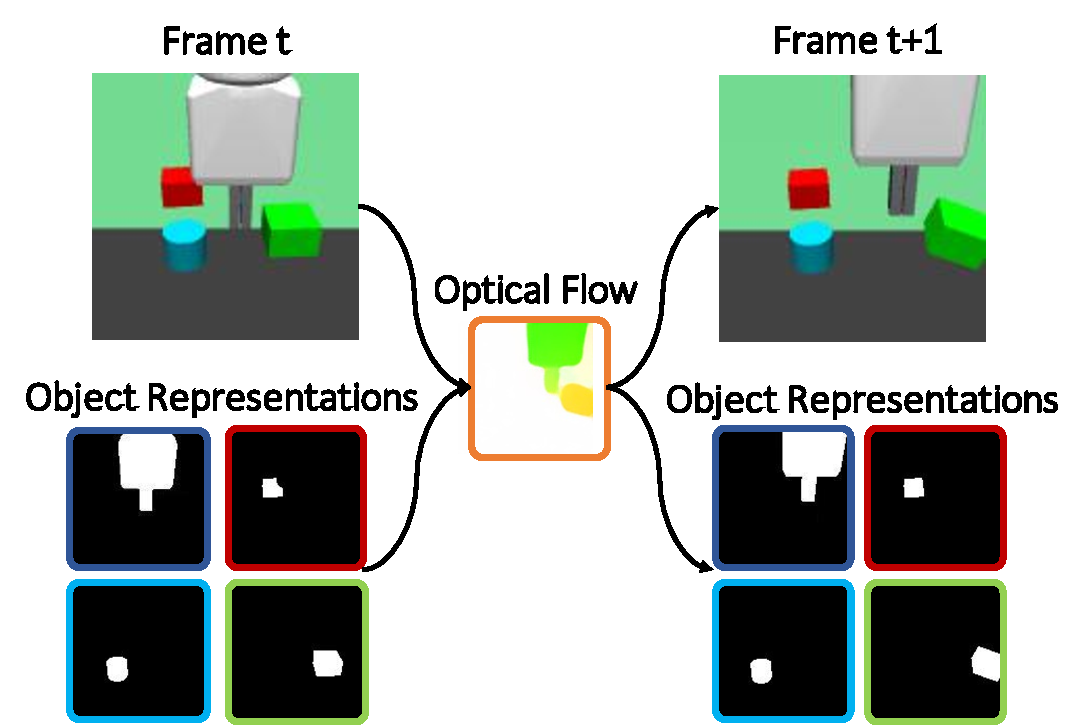
\includegraphics[width=8cm]{figs/flood_main_figure.pdf}
    \caption{Objects move as coherent wholes, therefore motions in natural video sequences preserve the object structure of the images, modulo minor boundary and occlusion effects. We identify the following simple desideratum for good discovered object-structured image representations such as the segmentation masks depicted here: object representations for nearby images in a video stream must be related to each other through the \emph{same optical flow warps} as the images themselves.}
    \label{fig:desired_property}
\end{figure}
%when objects move in an image stream generating a corresponding optical flow map between consecutive images, t
%Introducing the idea that an optical flow warp applied to an object-structured representation should produce the object-structured representation of the next image

We evaluate \textsc{flood} on a variety of synthetic object discovery benchmarks used in previous works. In addition, we introduce a real-world tabletop robotic object pushing dataset. Our results show that \textsc{flood} yields reliable improvements over baseline methods based on reconstruction and contrastive losses, and even an approach that has access to additional information about the forces causing object motions in video.



%This does not rely on specific encoder architectures.

%, identifying correspondences between pixels in consecutive frames

%This naturally implements the principle of common fate: pixels that move together belong together.


% --- loosely, warping the discovered segmentation map of frame A with optical flow should 

%, identifying correspondences between pixels in consecutive frames

%first proposed by Gestalt psychologists (CITE): common fate --- ``pixels that move together belong together''. 

%In this context, we call back to an older family of work within cognitive science and computer vision. 

%on representations learned in unsupervised visual representation learning.  

%inas imposing structure on unsupervised representaions

%relevant information for most tasks, : how might computer vision systems learn to parse their world into objects


%Gestalt psychologists studying the cognitive bases of grouping studied 

%Gestalt common fate

\section{Related Prior Work}
\label{sec:related_work}

%To move to after approach (?)

%Related work notes: 

\paragraph{Video object segmentation from motion and appearance.} As foreshadowed in Sec~\ref{sec:intro}, our approach for flow-guided object discovery is related to motion segmentation methods~\cite{shi1998motion,tron2007benchmark,yan2006general,tokmakov2017learning,keuper2018motion,bideau2018moa, yang2021rigidmask} in computer vision, which use optical flow cues to group pixels in video frames which move coherently together. Since purely flow-based groupings are not persistent and cannot handle static objects, video segmentation algorithms often combine these motion cues with appearance~\cite{weiss1995perceptually, jain2017fusionseg, tokmakov2017learning, cheng2017segflow}. However, all these methods are designed for segmenting video and can not handle static images as trained \textsc{flood} models do. Specifically, \textsc{flood} trains unsupervised appearance-based static image object segmentation models by using flow-based cues in training videos as a supervision signal.

% -- objects disappear once they stop moving. For more presistence, motion cues can be combined with appearance cues in video segmentation algorithms
%ALSO THE DEVA PAPER (?) 

\paragraph{Unsupervised representations from motion.} In the context of learning unsupervised representations, image region-level correspondences computed through object motion tracking~\cite{wang2015unsupervised} or by matching object-like regions~\cite{gao2016object} has been used before as a form of self-supervision. Compared to \textsc{flood}'s goal of discovering objects and forming object-structured representations of full images, they instead aim to train unstructured descriptors of objects and object-like regions in images. Most related to our approach from this literature, \citet{pathak2017learning} use motion segmentation of moving objects from video as targets for a single-image segmentation model. Note that this task is not well-posed; moving objects cannot be identified from a single image. Rather than produce a good segmentation model, this self-supervised segmentation task is merely intended as a ``pretext task''~\cite{pathak2017learning}, i.e., through training on this task, the CNN must acquire good unstructured image representations useful for other computer vision tasks.

%this is not a problem because they do not aim to train a segmentation model. Rather, 


\paragraph{Neural object discovery.} Nearly all neural object discovery approaches targeting general images or video are trained by reconstructing the input image~\cite{jakab2018unsupervised,jakab2020self,greff2019multi, burgess2019monet,locatello2020object,Kulkarni2019UnsupervisedLO, minderer2019unsupervised, engelcke2019genesis}. Some approaches use adversarial training: the idea is that object-structured representations can be modified and recomposed into valid images~\cite{chen2019unsupervised, yang2020learning}. Two recent approaches are trained through contrastive losses to distinguish between distinct images in a dataset~\cite{racah2020slot,lowe2020learning}. Among these, \citet{racah2020slot} use temporal continuity in video for object discovery, in a method called slot-contrastive networks (SCN). Like \textsc{flood}, SCN uses temporally nearby frames as positives and distant frames as negatives, but it effectively treats nearby images as being identical since it does not account for pixel motions. Instead, as specified above, \textsc{flood} models nearby frames as related by a warp specified by optical flow. We compare against SCN in Sec~\ref{sec:experiments}.  %also uses a loss from the contrastive family, but guided by optical flow. 

In robotics contexts, where motion is attributable to known robot actions, several models~\cite{kipf2019contrastive, kipf2018neural, Veerapaneni2019EntityAI} 
%\jd{Aurora, could you look into the Veerapaneni paper?} 
use action-conditioned future prediction as a training objective for joint object discovery and environment dynamics modeling. The robot actions in these formulations help specify how the scenes in training videos evolve over time. \textsc{flood} replaces robot actions with dense pixel correspondences from optical flow, which are more general --- they specify how arbitrary videos evolve even with unknown actors and forces. Notably, our implementation of \textsc{flood} uses the popular object slot encoder architecture of contrastive structured world models (C-SWM)~\cite{kipf2019contrastive}, enabling a controlled comparison in Sec~\ref{sec:experiments}. With identical object encoders, and sans robot action knowledge, \textsc{flood} still performs comparably or better than C-SWM even in robotics datasets with known actions.

% We do not assume robot action knowledge so that \textsc{flood} remains more general and able to learn from uncontrolled video.

%. However, since they do not directly reason about motions, they simply approximate consecutive frames as being identical
%However, these are philosophically close antecedents of \textsc{flood}.

%Learning object descriptors in an unsupervised manner through tracking~\cite{wang2015unsupervised,gao2016object}


% %\subsection{Object Discovery}  
% \begin{itemize}[leftmargin=*]
%     %\item  \textsc{flood} falls into this latter category.
    
%     %\item None of these above approaches use motion as a signal for discovering objects. In the robotics contexts, some models aim to discover both objects and their dynamics under robot action assuming that robot actions are known. 
    
%     %\item 
    
%     %In particular, \citet{kipf2019contrastive} proposes a contrastive structured world model (C-SWM), several of whose architectural components we borrow.
    
%     \item 
    
%     % \item IODINE
%     % \item MONET
%     % \item GENESIS
%     % \item Slot Attention
% \end{itemize}
% and that they are the only cause of motion in the scene

% \subsection{Contrastive Learning}
% \begin{itemize}
%     \item InfoNCE
%     \item SimCLR
%     \item Moco
% \end{itemize}
% \subsection{Flow-based Representation Learning Method}
% \begin{itemize}
%     \item Unsupervised Learning of Visual Representations using Videos
% \end{itemize}
% \subsection{Motion Segmentation}




\section{Flow-guided object discovery}
\label{sec:approach}

\paragraph{Task setup and motivation.} First, we introduce the unsupervised object discovery setting. Given a collection of unlabeled training images $\mathcal{D}$ that specify a visual domain, object discovery approaches aim to automatically identify the objects present among those images. For example, given images of toys in varied configurations on a cluttered tabletop, we would like to automatically discover those toys. Discovery is typically expressed by parsing or spatially disentangling new images from that domain and assigning some or all pixels to various discovered objects and background.
%including new images not within the training dataset $\mathcal{D}$, into their constituent objects. 

Object discovery is thus closely tied to the \emph{object-structured} representation in which the results of such image parsing are expressed. Indeed, training object discovery approaches amounts to learning unsupervised object-structured representations. Examples of such representations include keypoints~\cite{jakab2018unsupervised, Kulkarni2019UnsupervisedLO}, object detection bounding boxes~\cite{Cho_2015_CVPR}, segmentation masks~\cite{greff2019multi, kipf2019contrastive}, and skeletons capturing connected keypoints~\cite{jakab2020self}. Much research has focused on how to design innovative representations and infer them.
%As mentioned in Sec~\ref{sec:intro}, 

What are these representations useful for? Aside from having close correspondences with the \emph{true} objects in the scene, object-structured representations are intended to be compact, and to spatially disentangle the image into composable and coherently moving components. These properties are useful in downstream tasks such as robotics. For example, to model how visual scenes respond to robot actions, object-structured representations permit compact models in terms of how discovered object components interact with the robot and with each other~\cite{minderer2019unsupervised, Kulkarni2019UnsupervisedLO, kipf2019contrastive, lambeta2020digit} %(CITE Transporter, Minderer, DIGIT, C-SWM etc.).



 
% re-composition (moving objects around to produce a new scene) (CITE) or spatial dynamics modeling.

In the following subsections, we propose a new approach and training objective for neural object discovery. Prior approaches largely rely on image reconstruction, action-conditioned future prediction, or contrasting images in the training dataset, as we will discuss in Sec~\ref{sec:related_work}. Instead our approach, \textsc{flood}, uniquely mines supervisory signals from motions occurring in a training dataset of videos for learning to disentangle objects.  
% $\mathcal{D}$

\subsection{Slot representation and encoder}\label{sec:slots}
Our approach is not tied to only one choice of object-structured representation, but we ground our discussion and notation using \emph{``slot''} segmentation masks and vectors, which we will also use in experiments. An input image $x$, of size $H \times W$ pixels, is represented through a collection of $K$ \emph{slot} masks $ \bm{m}(x) = \{m^1(x), m^2(x), \dots. m^K(x) \}$  of size $H\times W$. All mask values lie between $0$ and $1$, i.e., $0 < m^k(i, j) < 1$ for all masks $k$, and pixel positions $(i, j)$. Masks $m^k(x)$ are intended to represent segmentation masks for objects in $x$. Each slot mask is then summarized as a $D-$ dimensional slot vector $z^k(x)$. $\bm{z}(x)$ represents all $K$ slot vectors combined. In our work, each slot is free to bind to any object or background in the input image.\footnote{This is not true in \citet{kipf2019contrastive}, due to the requirement of object-specific actions for each slot.}

%What is the structure of the function that produces this representation? 
How are these slot masks and vectors generated from input images? We use the popular neural network architecture proposed in \citet{kipf2019contrastive}. An ``object extractor'' convolutional neural network $\mathcal{F}$ with a sigmoid output layer produces $K$ convolutional maps constrained to lie in $[0, 1]$. These represent the slot masks $ \bm{m}(x)$. Next, a small multi-layer perceptron $\mathcal{G}$ processes each flattened slot mask to produce its corresponding slot vector: $z^k(x)$. This compression serves as a representational bottleneck that encourages the emergence of object-structured representations, as we will discuss below. The second and third rows of Fig~\ref{fig:architecture} illustrate this procedure.

% by a softmax activation functio
%, which we also use in our experiments
 
%The segmentation masks are of the same size as input images take values between $0$ and $1$, 

%Specifically, \textsc{flood} takes in an image input $f_t$, which is the video frame at time step $t$, and passing it through an object discovery network. This discovery network produces a set of feature maps $m_t = \{m_{t}^1, m_{t}^2, \dots. m_{t}^k \}$ around the discovered objects, where $k$ is the number of objects we expected. 



%At a high level, all unsupervised object discovery approaches aim to produce representations that are: compact, spatially disentangled, interpretable, permit composition (CITE IODINE/MoNET, and the GAN papers) and spatial reasoning. This in turn can be useful for downstream applications such as robotics, in modeling how visual scenes respond to robot actions simply through modeling the responses of discovered objects. (CITE Transporter, Minderer, DIGIT, C-SWM etc.) 

%This identification is typically expressed through a simple 

\begin{figure}
  \centering
  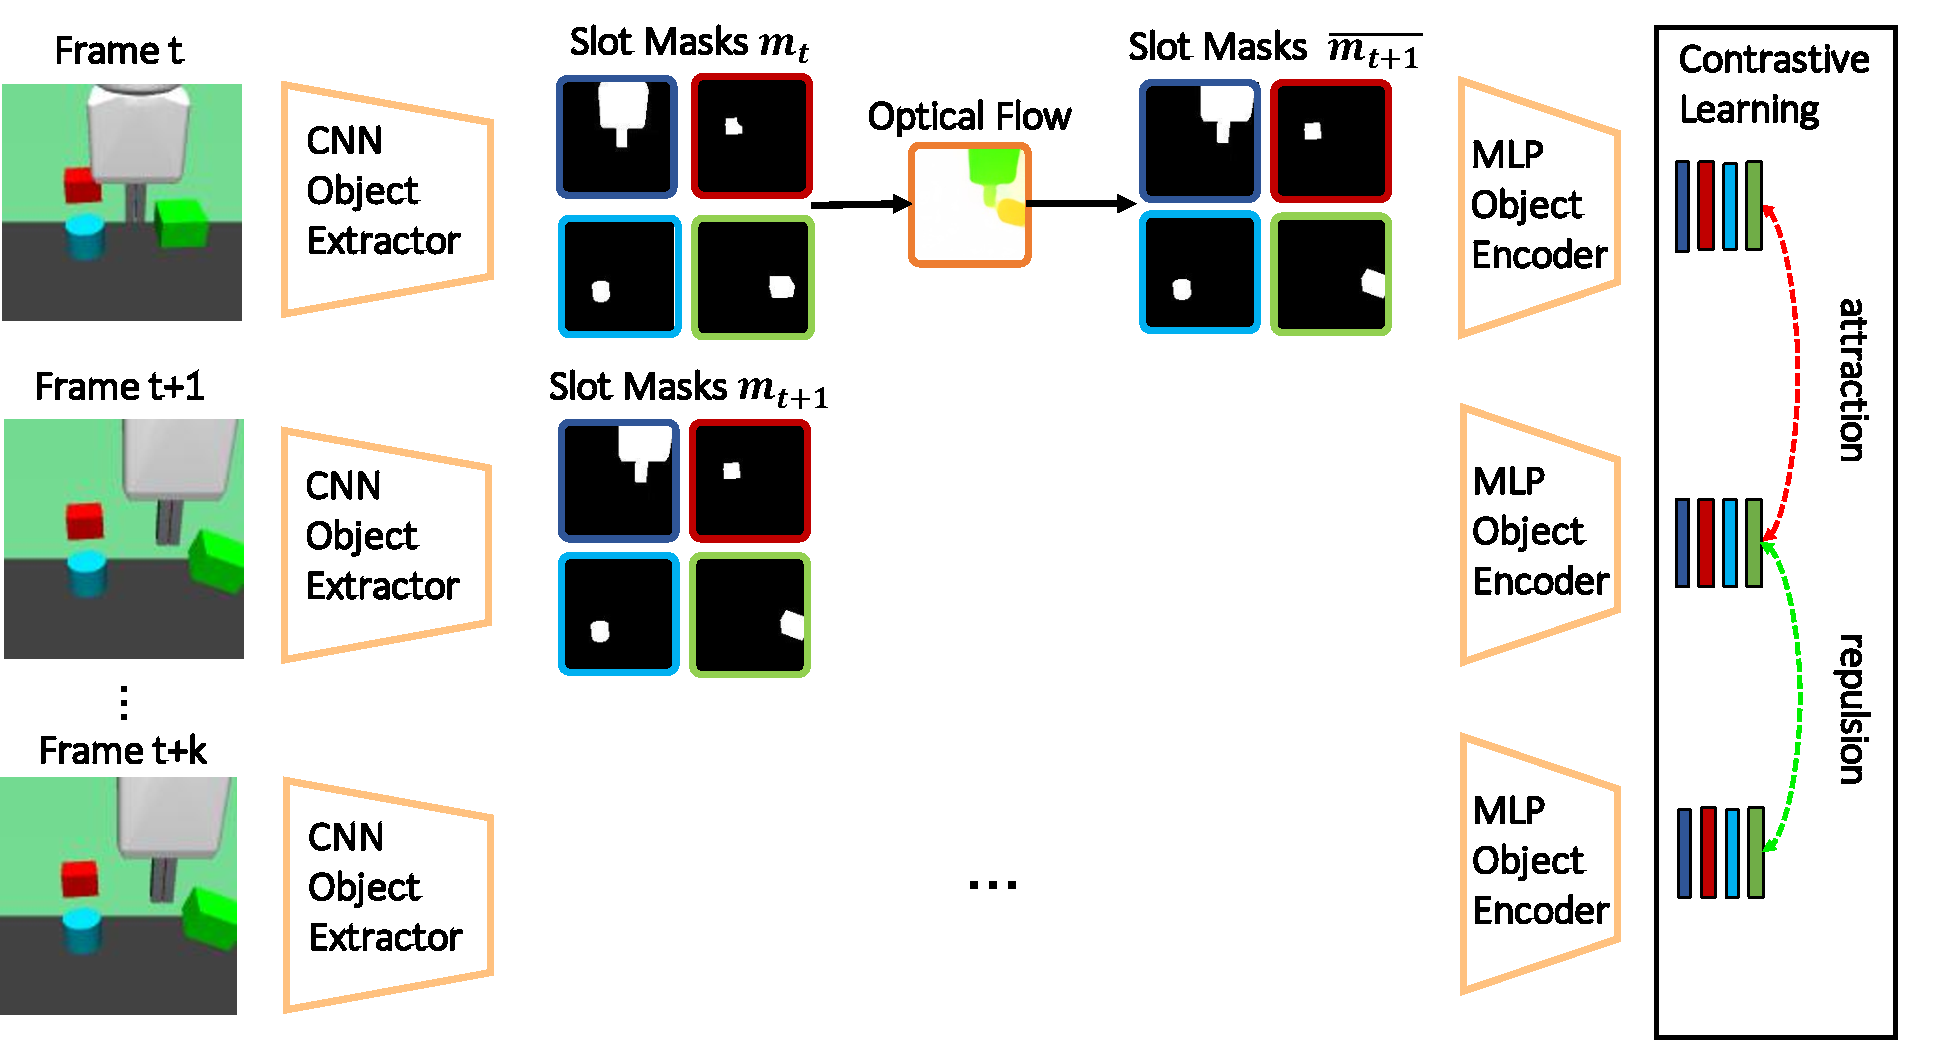
\includegraphics[width=14cm]{figs/flood-network.pdf}

  \caption{The training setup for \textsc{flood} (Sec~\ref{sec:flood}), applied to object-structured slot representations (Sec~\ref{sec:slots}).}
  \label{fig:architecture}
\end{figure}

%\jd{Suggestion for how to structure this: First, set up the problem and notation. What is given to you, and what is the goal? Then describe the slot encoder architecture and how objects are represented in slots. Should state that this is the representation used in C-SWM and resembles the representations used in other work. Our method is also compatible with other object representations, but we use this popular representation in our implementations. Next, we describe the desired property of those representations in terms of pixelwise flow i.e. warp ( mask ( frame 1)) = mask ( warp (frame 1)), where  warp(frame 1) = frame 2, and the warp is computed from optical flow. Next, we describe how this can be implemented using contrastive losses.}

\subsection{Optical flow, and how motions can help with object discovery} \label{sec:flow}

An important characteristic of objects, known for long to be particularly useful for object grouping, is that objects move as coherent wholes. This idea has been known for at least a century, and is captured in the pithy Gestalt~\cite{wertheimer1938laws} phrase: ``pixels that move together group together.'' 
%, barring rare exceptions such as disintegration

Yet, to our knowledge, no existing approaches for neural object discovery use this information, including many that train on video sequences, such as~\cite{racah2020slot, jakab2018unsupervised, kipf2019contrastive}. %We too train on video sequences, but 
We address this gap by proposing a novel approach to use the coherent motions of objects in training videos as training signals to guide %$\mathcal{F}$ and $\mathcal{G}$ to perform 
object discovery. %We call this ``flow-guided object discovery''

Our key idea is illustrated in Fig~\ref{fig:desired_property}. Objects move as coherent wholes, and the objects in two neighboring images in video are the same, only (possibly) slightly displaced. Therefore, our slots (generalizable to other object-structured representations) should satisfy the following desiderata: %\jd{could fold into text if need be, for space}
\begin{itemize}[leftmargin=*]
 \item Slots should bind to the same set of objects in both frames. 
 \item Slots should be sensitive to the small changes in the \emph{positions} of those objects. In particular, each slot mask $m^k$ should exactly track the displacement of the object that it is bound to.
\end{itemize}

%\paragraph{The \textsc{flood} algorithm. } 
To frame these desiderata as a mathematical objective, we introduce the concept of \emph{optical flow}. An optical flow field  $h_{a\rightarrow b}$ defines a warp between images $a$ and $b$, such that $b=h_{a\rightarrow b}(a)$ . In other words, $h_{a\rightarrow b}$ specifies a displacement for each pixel in $a$, such that the resulting image is equal to $b$. Optical flow computation is a well-studied problem in computer vision, and many mature solutions exist. We use FlowNet2.0~\cite{flownet2}, which is trained on four large synthetic datasets of animated object videos~\cite{flying3d, flyingchair,chairsd,sintel}. %\jd{like FlyingThings, or exactly FlyingThings?}
%there are many existing off-the-shelf approaches for optical flow field computation. 
%Note that the optical flow field is not unique, and indeed, video frames with large ``flat'' regions of the same color permit many compatible flow fields. 

%We treat the optical flow field as 
The optical flow field $h_{x\rightarrow x'}$ provides us with correspondences between pixels in temporally nearby frames $x$ and $x'$.  
%Given the optical flow field $h_{x\rightarrow x'}$, 
Now, the desiderata for slots, stated above, boil down to requiring that the pixel correspondences between neighboring frames $x$ and $x'$ are preserved in the correspondences between their slot masks $m^k(x)$ and $m^k(x')$. For all slot indices $k$:
\begin{equation}
    h_{x\rightarrow x'}(m^k(x)) = m^k(x'). \label{eq:desideratum}
\end{equation}
In other words, if $m^k(x)$ is a good segmentation mask for \emph{some} object in image $x$, then it maps to the next timestep through the same optical flow warp as the input images themselves. %Eq~\eqref{eq:desideratum} is the flow-guided object discovery (\textsc{flood}) desideratum. 

%It is easy to see that how these masks map to the same 
%Yet anothe way to state this is: (correct) segmentation is equivariant to object motion:  $h_{x\rightarrow x'}(m^k(x)) = m^k(h_{x\rightarrow x'}(x))$.

%Or, the pixel correspondences between images are also correspondences between the slot masks.

%$m^k(x)$

%expressed for slot masks 
This simple optical flow-based desideratum implicitly exploits the fact that objects in video move coherently, in ways that preserve their identity. To see this, observe that Eq~\eqref{eq:desideratum} would \emph{not} hold true for good slots $m^k$ and arbitrary warps $h$. For example, $h$ might move all pixels in $x$ by random displacements. In this case, the resulting image $x'$ would no longer plausibly retain the object identities present in $x$, and $m^k(x')$ cannot therefore be expected to preserve them either. Optical flow warps corresponding to frames in natural videos are thus special, in that they are object identity-preserving.

As a sidenote, in the above discussion, we have largely assumed that optical flow masks provide perfect pixel correspondences between the same real three-dimensional particle in nearby frames $x$ and $x'$. Optical flow methods, while they perform very well in our experiments, do of course only produce noisy correspondences. However, as our experimental results validate, this is not a major concern.

%\jd{Slightly uncomfortable about the fact that this all speaks of optical flow as if it provides some ground truth correspondence .. e.g. what happens if the illumination changes suddenly, and flow correspondences become weird? More broadly, should we say something about the fact that the correspondences are based on low-level appearance properties, and may only be noisy versions of the true 3D point correspondences?}

%Thus, the above mathematical statement of the desiderata exploits the fact that objects move coherently, in ways that preserve their identity. 

%Note that this is not true for arbitrary wraps of the inputs

%In other words, the segmentation mask 

%Objects move as coherent wholes, therefore motions in natural video sequences preserve the object structure of the images, modulo minor boundary and occlusion effects. We identify the following simple desideratum for good discovered object-structured image representations such as the segmentation masks depicted here: object representations for nearby images in a video stream must be related to each other through the \emph{same optical flow masks} as the images themselves.

%Specifically, while prior work has trained OS representations from objectives 

%~\cite{tron2007benchmark,yan2006general,keuper2018motion,bideau2018moa, yang2021rigidmask}

%A natural way to collect the training image dataset $\mathcal{D}$ is to gather images from the frames of video. 

%Given some unlabeled video sequences, the goal of our method is to discover and learn object-centric representations with the help of motion information. Specifically, \textsc{flood} takes in an image input $f_t$, which is the video frame at time step $t$, and passing it through an object discovery network. This discovery network produces a set of feature maps $m_t = \{m_{t}^1, m_{t}^2, \dots. m_{t}^k \}$ around the discovered objects, where $k$ is the number of objects we expected. 

% In order to take advantages of the motion information available in a video, \textsc{flood} takes in motion information provided by optical flow between two nearby frames $f_{t}$ and $f_{t'}$, and propagates the predicted feature maps $m_{t}$ to $\overline{m_{t'}}$. If the optical flow between these two frames are correct, we should expect that $\overline{m_{t'}}$ and $m_{t'}$ encodes the same object information. We could then use this property to train our object discovery network.

% In this section, we first introduce our object discovery network. Next we describe our desired property of the learned representations in terms of optical flow. In the end we explain how to use these desired properties to train the object discovery network through contrastive learning. 

% \subsection{Object-structured representation}
% The object discovery network $N_D$ takes in an image $f_t$, and outputs a set of $k$ feature maps $N_D(f_t) = m_t = \{m_{t}^1, m_{t}^2, \dots. m_{t}^k \}$. This networks is an CNN-based network, and the last activation layer is a sigmoid function. Thus each mask can be interpreted as a slot-wise segmentation mask that takes the value between 0-1. This slot-wise object representation is also used in ~\cite{kipf2019contrastive, locatello2020object}. Since it's a popular object representation in previous work, we adopt this in our implementation. \aq{I am afraid that if we say out method is also compatible with other object representations, reviewers are going to ask for results on other representations}

% \subsection{Flow-guided object discovery propagation}
% As mentioned above, we believe that motion information in nearby video frames contain critical training signal for object discovery tasks. More specifically, given two nearby video frames $f_{t}$ and $f_{t'}$, the optical flow defines a map between frames: $h_{t \rightarrow t'}(f_t) = f_{t'}$ and $h_{t' \rightarrow t}(f_{t'}) = f_{t}$. This map defines a morphism and we can use it to propagate object information from one frame to another:
% \[h_{t \rightarrow t'}(N_D(f_t)) = N_D(h_{t \rightarrow t'}(f_t))\],
% where $h_{t \rightarrow t'}(N_D(f_t)) = \overline{m_{t'}}$ and $ N_D(h_{t \rightarrow t'}(f_t)) =  N_D(f_{t'}) = m_{t'}$.

% If this morphism holds, then we know the following two conditions hold:  1) the map between frames($h_{t \rightarrow t'}$) is accurate, and 2) the object discovery feature maps are consistent across frames. The first condition is given by the precision of optical-flow prediction network. The second condition coincide with the training objective of our object discovery network. We next describe how to enforce this second condition via contrastive learning.

\subsection{The \textsc{flood} training objective}\label{sec:flood}

%In targeting the desiderata of Eq~\ref{eq:desideratum}, there are two degenerate solutions we would like to avoid
The desideratum in Eq~\eqref{eq:desideratum} cannot directly be set up as a training objective, since it permits two degenerate solutions: $m^k(x)=\bm{0}$ for all $x, k$, (``all-zeros'' ), and  $m^k(x)=x$ for all $x$ (``identity''). We avoid these by defining a contrastive training objective over the slot vectors $\bm{z}(x) = \mathcal{G}(\bm{m}(x))$. 

%Following the success of contrastive objectives for unsupervised representation learning (CITE CPC, SIMCLR etc.), we set up a contrastive objective to achieve Eq~\ref{eq:desideratum}. % using contrastive objectives 

Let $\overline{\bm{m}(x')} \triangleq h_{x \rightarrow x'}(\bm{m}(x))$ represent the prediction of the slot mask $\bm{m}(x')$ obtained by flow-warping $\bm{m}(x)$. Note that this is the LHS of Eq~\eqref{eq:desideratum}, combined over all slot indices $k$.  Now, let $\overline{\bm{z}(x')}=\mathcal{G}(\overline{\bm{m}(x')})$ represent its corresponding predicted slot vectors. 

Then, the flow-guided object discovery (\textsc{flood}) objective is:
\begin{equation}
\mathcal{L} = \exp \dfrac {d(\overline{\bm{z}(x')}, \bm{z}(x'))}{\sum_{x^-} d(\bm{z}(x), \bm{z}(x^-)}, \label{eq:flood_loss}
\end{equation}
where $d(\cdot, \cdot)$ is a distance function between slot vectors, and $x^-$ are negatives for $x$. Similar to prior works in unsupervised contrastive representation learning~\cite{oord2018representation,chen2020simple}, this may be interpreted as a softmax classification objective for distinguishing the positive pair (in the numerator) from negative pairs (in the denominator). We set $d$ to be the summed $\ell_2$ error over slots, and the negative frames $x^-$ are uniformly drawn from frames that are more than $T=1$ steps away from the current frame $x$ in the training videos. 
%\jd{Check this for inaccuracies}. 
Recall that $x$ and $x'$ are temporally nearby frames, yet the positives above are not directly their corresponding slot vectors $\bm{z}(x)$ and $\bm{z}(x')$. Instead, the slots of $x$ are first warped through the optical flow warp to compute $\overline{\bm{z}(x')}$, as motivated in Sec~\ref{sec:flow}.

This contrastive objective trivially precludes the all-zeros degenerate solution above. Avoiding the ``identity'' solution is more subtle: it is done by applying the contrastive loss to a compressed representation $\bm{z}=\mathcal{G}(\bm{m}(x))$, computed by a small MLP $\mathcal{G}$. The low capacity of $\mathcal{G}$ means that it should be very easy to extract a small code $\bm{z}$ that is sufficiently discriminative to minimize Eq~\ref{eq:flood_loss}. This forces the network to only represent only highly processed information in the masks $m^k$, thus avoiding the identity mapping $m^k(x)=x$. 

\subsection{Implementation Details}

%Lastly we describe some network implementation details. 
In our experiments, the object extractor $\mathcal{F}$ is a four-layered convolutional neural network. The first three convolutional layers are followed by a relu and a batchnorm layer. The last convolutional layer is followed by a sigmoid, so that the predicted slot masks $\bm{m}(x)$ lie in $[0,1]$.  %, with a 3 x 3 kernels on each layer This convolutional neural network $\mathcal{F}$ is followed by a 
The object encoder $\mathcal{G}$ is a small multi-layer perceptron 
%that takes in flattened slot masks $m^k(x)$ and produced slot vectors $z^k(x)$. $\mathcal{G}$ 
consisting of three layers, with a LayerNorm~\cite{LayerN} between the second and the third MLP layer. We use the Adam optimizer and train this network on a single 2080Ti GPU with batch size of 1024. 

There are two main hyperparameters in our method: slot vector dimension and slot number. For all experiments with our method, we fix the slot number to six. We keep all the other training hyperparameters as well as slot vector dimension as the same from C-SWM.


%\jd{Need to talk about how both degenerate solutions are avoided?}

% \jd{needs to be written out as a softmax over positives and negatives}

%combined LHS in Eq~\ref{eq:desideratum} for all mask indices $k$

%Our general goal is to make sure that object representations $m_t$ from different frames are consistent with each other, i.e. that each slot of the learned feature map should represent a consistent object. 
% In order to achieve this goal, we first propagate the learned feature map of frame $t$ into a nearby frame $t'$: $\overline{m_{t'}} = h_{t \rightarrow t'}(N_D(f_t))$. Next we want to enforce the consistency on $\overline{m_{t'}}$ and $m_{t'}$. Doing so directly on feature maps would be too costly, thus we encode the learned feature maps $m_t$ using an 3-layer MLP $N_E$ into a latent embedding $z_t$. Finally we formalize our goal in a constrastive learning objective:
% \[\mathcal{L} = d(N_E(m_{t'}),N_E(\overline{m_{t'}}))\]



\section{Experiments}
\label{sec:experiments}

Our experiments aim to answer the following questions: \textbf{(1)} How well does \textsc{flood} with slot representations perform against representative state-of-the-art approaches from various families of neural object discovery algorithms? \textbf{(2)} How does \textsc{flood} compare against ablations that use the same architecture, but with different training objectives? \textbf{(3)} While most past work on neural discovery has been evaluated in simplistic settings, can \textsc{flood} handle real-world images set in a plausible robotics application?

%When controlling the representation, how well does 

\subsection{Baselines and Ablations}\label{sec:baselines}

Throughout our experiments, we compare against three recent baselines, representing different types of object discovery objectives from the literature. 

\begin{itemize}[leftmargin=*]
 \item Contrastive structured world model (\textbf{C-SWM})~\cite{kipf2019contrastive} represents methods for joint object discovery and environment dynamics modeling trained through an action-conditioned future prediction objective. Compared to our method and other baselines, it requires extra information about object-specific actions at each instant. 
 \item  Slot attention (\textbf{SA})~\cite{locatello2020object} represents object discovery through image reconstruction, using a new attention-based architecture to encode images into slots. It produces slot masks, but does not have a direct analogue of slot vectors used in our approach. 
 \item  Finally, slot-contrastive networks (\textbf{SCN})~\cite{racah2020slot}, discussed above in Sec~\ref{sec:related_work}, use temporal continuity for object discovery: like \textsc{flood}, it trains representations that can distinguish far-away frame pairs from nearby frame pairs using a contrastive loss, but it does not use optical flow correspondences between nearby frames. SCN directly produces slot vectors without first generating slot masks.
\end{itemize}
% as discussed in Sec~\ref{sec:related_work}

\textsc{flood} inherits the object extractor and object encoder of C-SWM, which is also used in SCN, making it particularly well-suited for comparison. To enable a more controlled comparison of object discovery approaches with a fixed architecture, we create two ablations of our method that use an SCN-like ``temporal continuity'' objective, and another that uses an SA-like image ``reconstruction'' objective. Since C-SWM already shares the same architecture, it doubles up as the third ablation, representing a ``dynamics modeling'' objective. %\jd{Use these names in the table, or change these names.}

%SA proposes a new attention-based architecture for encoding images into object slots.

%All three baselines represent objects through a slot-based representation similar to \textsc{flood}, described in Sec~\ref{sec:approach}, making them well-suited for direct comparison. \textsc{flood} inherits the object encoder of C-SWM, which is also used in SCN. SA proposes a new attention-based architecture for encoding images into object slots.


\subsection{Datasets}
%\jd{If space, a figure up front just displaying a collection of images from each dataset to illustrate their corresponding visual domains.}
\begin{figure}
\begin{subfigure}{.3\linewidth}
\centering
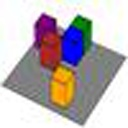
\includegraphics[width=2.5cm]{figs/cubes.jpg}
\caption{}
\label{fig:sub1}
\end{subfigure}%
\begin{subfigure}{.3\linewidth}
\centering
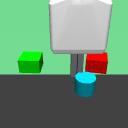
\includegraphics[width=2.5cm]{figs/sim.jpg}
\caption{}
\label{fig:sub2}
\end{subfigure}
\begin{subfigure}{.3\linewidth}
\centering
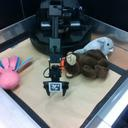
\includegraphics[width=2.5cm]{figs/real.jpg}
\caption{}
\label{fig:sub3}
\end{subfigure}
\caption{Sample images from the three datasets (a) \textbf{CUBES}, (b) \textbf{SIM}, and (c) \textbf{REAL}.}
\label{fig:datasets}
\end{figure}
We evaluate \textsc{flood} on three video datasets: 
\begin{itemize}[leftmargin=*]
    \item \textbf{CUBES} is a 3D blocks dataset, adopted from \citet{kipf2019contrastive}. This is a grid-world environment with discrete actions applied to selected blocks, such as ``move object 1 one step forward'' and ``move object 2 one step left''). We use the authors' code to collect a video dataset with a random action policy, using identical settings as in \citet{kipf2019contrastive}. We train on 1000 training videos of length 100 frames each, and evaluate on 10,000 videos of length 10. All frames are 50x50 RGB images. The robot executes a new action in each frame. For C-SWM, object-specific actions are provided as a four-dimensional one-hot vector(if an action is applied to that object) or a vector of zeros for each object slot.
    \item \textbf{SIM} is collected in a custom new simulated robotic manipulation environment. We use MuJoCo~\cite{todorov2012mujoco} to render a tabletop with three simple object shapes (a green cube, a red cube, and a blue cylinder) and a Fetch robot. We collect 1000 training videos and 1000 testing videos, all of length 15 frames, involving 15 separate robot motions. In each episode, the robot randomly picks one object and a direction to push it to.  All frames are 128 x 128 RGB images. For C-SWM, object-specific actions are provided as a two-dimensional vector(if an action is applied to that object) or a vector of zeros for each object slot.
    \item \textbf{REAL} is analogous to \textbf{SIM}, but collected on a real robot arm, and with more complex objects and dynamics. We use a WidowX 200 robot arm and three deformable toys. The videos involve the robot performing random end-effector motions in each frame, colliding frequently with the objects and displacing them. We collect 350 training videos, and evaluate on 50 videos, all of length 30. All frames are 128 x 128 RGB images. For C-SWM, object-specific actions are provided as a five-dimensional vector(if an action is applied to that object) or a vector of zeros for each object slot.
\end{itemize}

We will publicly release all datasets and code. Sample frames from all datasets are shown in Fig~\ref{fig:datasets}.

%, collected from various environments
%The first one is a 3D blocks pushing dataset (\textbf{CUBES}), which is adopted from C-SWM. This is a grid-world environment with discrete actions. We use a random policy to collect observation data of size 50 x 50 x 3. 

%The second environment is a simulated control environment (\textbf{SIM}). In this environment, we use Mujoco to render a tabletop with three rigid objects. Before each episode, we randomly initialize the robot start location as well as position and orientation of those three rigid objects. We use a random policy to select which block to push at the start of each episode.  The observation is provided as 128 x 128 x3 images, looking down at the table top.

%The third environment is a photo-realistic control environment (\textbf{REAL}). For this environment, we use a locobot to collect object pushing data. In this environment, we have three non-rigid objects on the table. We use a random policy to collect robot-object interaction data. We use an external webcam to capture the observations, each of size 128 x 128 x 3.

% \subsection{Training and Evaluation Settings}
% For \textbf{CUBES}, we generate 1000 training episodes with 100 environment steps, and 10000 evaluation episodes with 10 environment steps.  
% For \textbf{SIM}, we generate 1000 training episodes and 1000 evaluation episodes, each of them containing 15 enviornmental steps.
%For \textbf{REAL}, we generate 400 episodes, each with 30 steps. We keep 350 episodes for training and 50 for evaluation.


\subsection{Quantitative Evaluation Metrics}

We use two evaluation metrics for our slot representations: %\jd{highlight ARI more than MSE, since it is more standard. Also put it first in the tables. Use KLME, defined below, instead of MSE.}
%In order to evaluate the quality of learned object representations, we adopt two evaluation metrics. 
\begin{itemize} [leftmargin=*]
    \item \textbf{ARI}: To evaluate the slot masks as object segmentation masks, we adopt a widely used metric for multi-object segmentation: Adjusted Random Index(ARI)~\cite{ari1,ari2}. ARI measures the similarity of two groupings of pixels, and is invariant to the permutation of groupings. We compare the set of slot masks produced by slot encoder with ground truth object segmentation masks.  %(excluding the background mask)
    \item \textbf{KLME}: While ARI evaluates slot masks, it does not directly evaluate the slot vectors. To do this, we define a new metric as follows. We train $NK$ linear regression models $f_{nk}$, one to regress each of the $K$ slot vectors to each of $N$ ground-truth 2D object coordinates in the scene, corresponding to specific keypoints on $N$ objects. For each object $n$, we select $\min_k \text{MSE}_n(f_nk)$
    %the slot $k^*(n)$ that minimizes the linear regression mean-squared error on held-out data, and use $\text{MSE}_n (f_{nk^*(n)})$ 
    as a score that captures how well that keypoint is represented, where $\text{MSE}_n$ is the linear regression mean squared error on held-out data. This corresponds to finding the closest-matching slot for each keypoint, and measuring how well they match. 
    Averaging this score over all $N$ keypoints produces our keypoint location matching error (KLME) metric for slot vectors.  %take the model with the lowest error across all slots prediction with the lowest error across all slots and measure the MSE loss on predicted 2D pixel location of each object. 
    %This metric allows us to directly measure the quality of learned slot vectors.
\end{itemize}

Ground truth object segmentation masks and keypoint locations are readily available in the simulated environments.  
%In order to measure the above two metrics, we generate ground truth segmentation mask and 2D ground truth location for each object in the observation. 
For \textbf{REAL}, we labeled segmentation masks for 90 test images, and 2d location of objects for 660 test images, to permit the measurement of ARI and KLME respectively.

Note that SA does not produce slot vectors, so we omit its KLME in our quantitative results. Likewise, SCN does not produce slot masks, so we omit its ARI.

%uses a new attention-based architecture to encode objects, and 

% \textbf{C-SWM}\\
% \textbf{Slot Contrastive Networks}\\
% \textbf{Slot Attention}


%\subsection{Experiment Setup}

\subsection{Results}
\setlength{\tabcolsep}{20pt}
\renewcommand{\arraystretch}{1.5}


\begin{table}[t]
  \caption{Quantitative comparison against published baselines. Best performance in \textbf{bold}}
  \label{table:main-result}
  \centering
  \resizebox{\textwidth}{!}{
  \begin{tabular}{llllll}
    \toprule
       & & \textbf{\textsc{flood}(Ours)}      & \textbf{C-SWM}~\cite{kipf2019contrastive}    & \textbf{SCN}~\cite{racah2020slot}     & \textbf{SA}~\cite{locatello2020object}  \\
    \midrule
    \multirow{2}{*}{\rotatebox[origin=c]{90}{\textbf{SIM}}} & \textbf{ARI(\%)$\uparrow$}     &  \textbf{93.56}  & 70.93  & - &  50.07 \\
    \cmidrule(r){2-6}
    &  \textbf{KLME$\downarrow$}  & \textbf{100.86} &  \textbf{99.61}  &286.18 &   -   \\
    \midrule
    
     \multirow{2}{*}{\rotatebox[origin=c]{90}{\textbf{REAL}}} &\textbf{ARI(\%)$\uparrow$}      & \textbf{16.86}  &  \textbf{15.97}  & - &  10.20  \\
    \cmidrule(r){2-6}
    & \textbf{KLME$\downarrow$} & \textbf{786.48}& 830.34&  806.73   &   -   \\
    \midrule
    
      \multirow{2}{*}{\rotatebox[origin=c]{90}{\textbf{CUBES}}}&\textbf{ARI(\%)$\uparrow$}     & 85.51  &   \textbf{95.09} & - & 85.29  \\
    \cmidrule(r){2-6}
        & \textbf{KLME$\downarrow$}  & 59.92 &  \textbf{54.79}  & 332.42 &   -   \\
    \bottomrule
  \end{tabular}
  }
\end{table}

Table~\ref{table:main-result} summarizes results for our method and the baselines on all three datasets. 
Our method easily outperforms SA and SCN, and performs comparably with C-SWM, which has access to additional information about object actions at each step. In particular, C-SWM  shines on \textbf{CUBES}, the simplest environment, where object-specific actions are discrete and cleanest. 

Table~\ref{table:objective} shows results of the objective function ablations of our approach mentioned above in Sec~\ref{sec:baselines}, with network architecture fixed. These results are reported on on \textbf{SIM}, which has clean annotations of object segmentations and keypoints for evaluation. 
%We show results for a controlled comparison of object discovery approaches in . For this experiment, we fix the object discovery network structure, and only change the training objective. 
%In addition to the training objective used in our method, we adopted three other objectives: "dynamics modeling", "temporal continuity" and "reconstruction" from our baseline methods. 
Once again, we easily outperform the baselines, illustrating that the flow-guided objective is important to our method's overall performance. 
%Our training objective performs the best in terms of ARI, illustrating that our training objective produces the best quality slot masks comparing to all the other three baselines.

%In both \textbf{SIM} and \textbf{REAL}, where the action labels are continuous, our method out performs all the other three baselines in terms of slot mask prediction quality. 
%In general, we observe that our method compares favorably against the other three baselines. Our method's performance in \textbf{CUBES} is slightly worse than our baseline C-SWM. However, it is worth noting that \textbf{CUBES} is a relatively simple environment and the discrete action label is available at training time for C-SWM. In both \textbf{SIM} and \textbf{REAL}, where the action labels are continuous, our method out performs all the other three baselines in terms of slot mask prediction quality. 

Fig~\ref{fig:qual_sim} and~\ref{fig:qual_real} show examples of masks produced by \textsc{flood} and baselines for two images per dataset. 
For each object in the scene, we show the mask that most frequently binds to it. 
Some methods do not successfully bind to all objects in the scene; for them, we do leave empty spaces representing missing slots.
More extensive results, including all slot masks produced by each method, are shown in Supp.



\begin{figure}
  \centering
  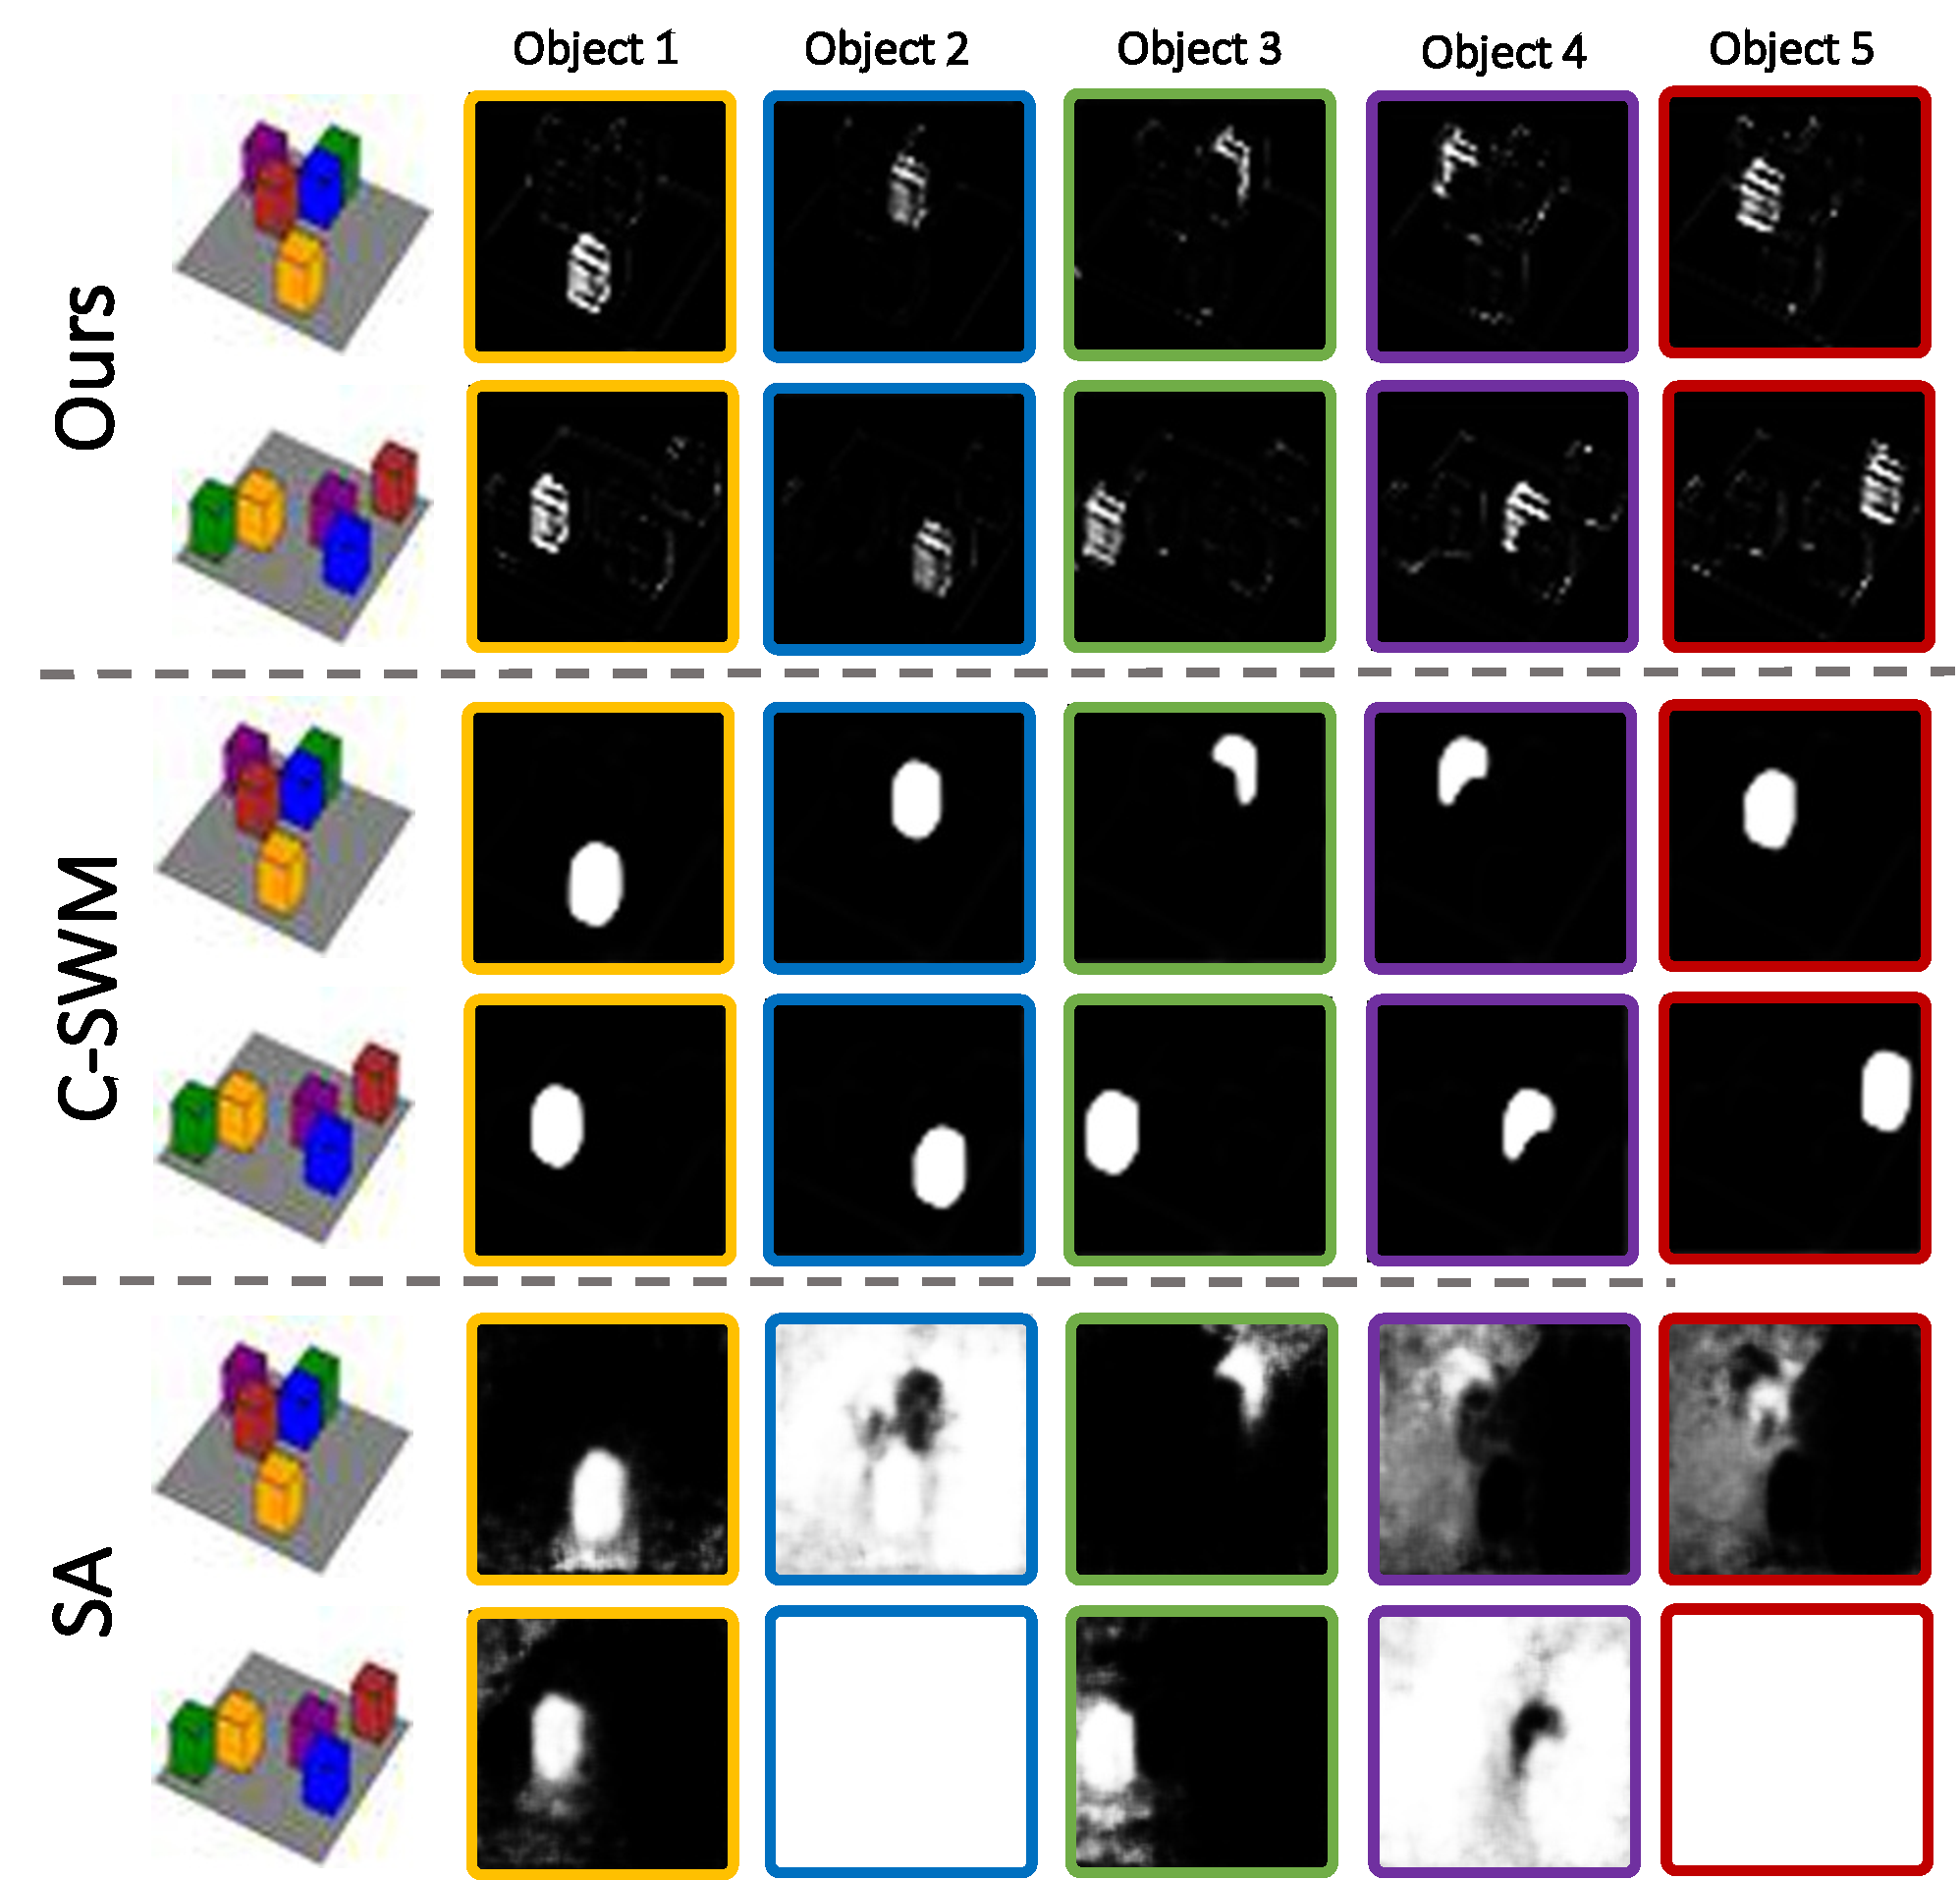
\includegraphics[height=0.3\textheight]{figs/qual_cubes.pdf}
  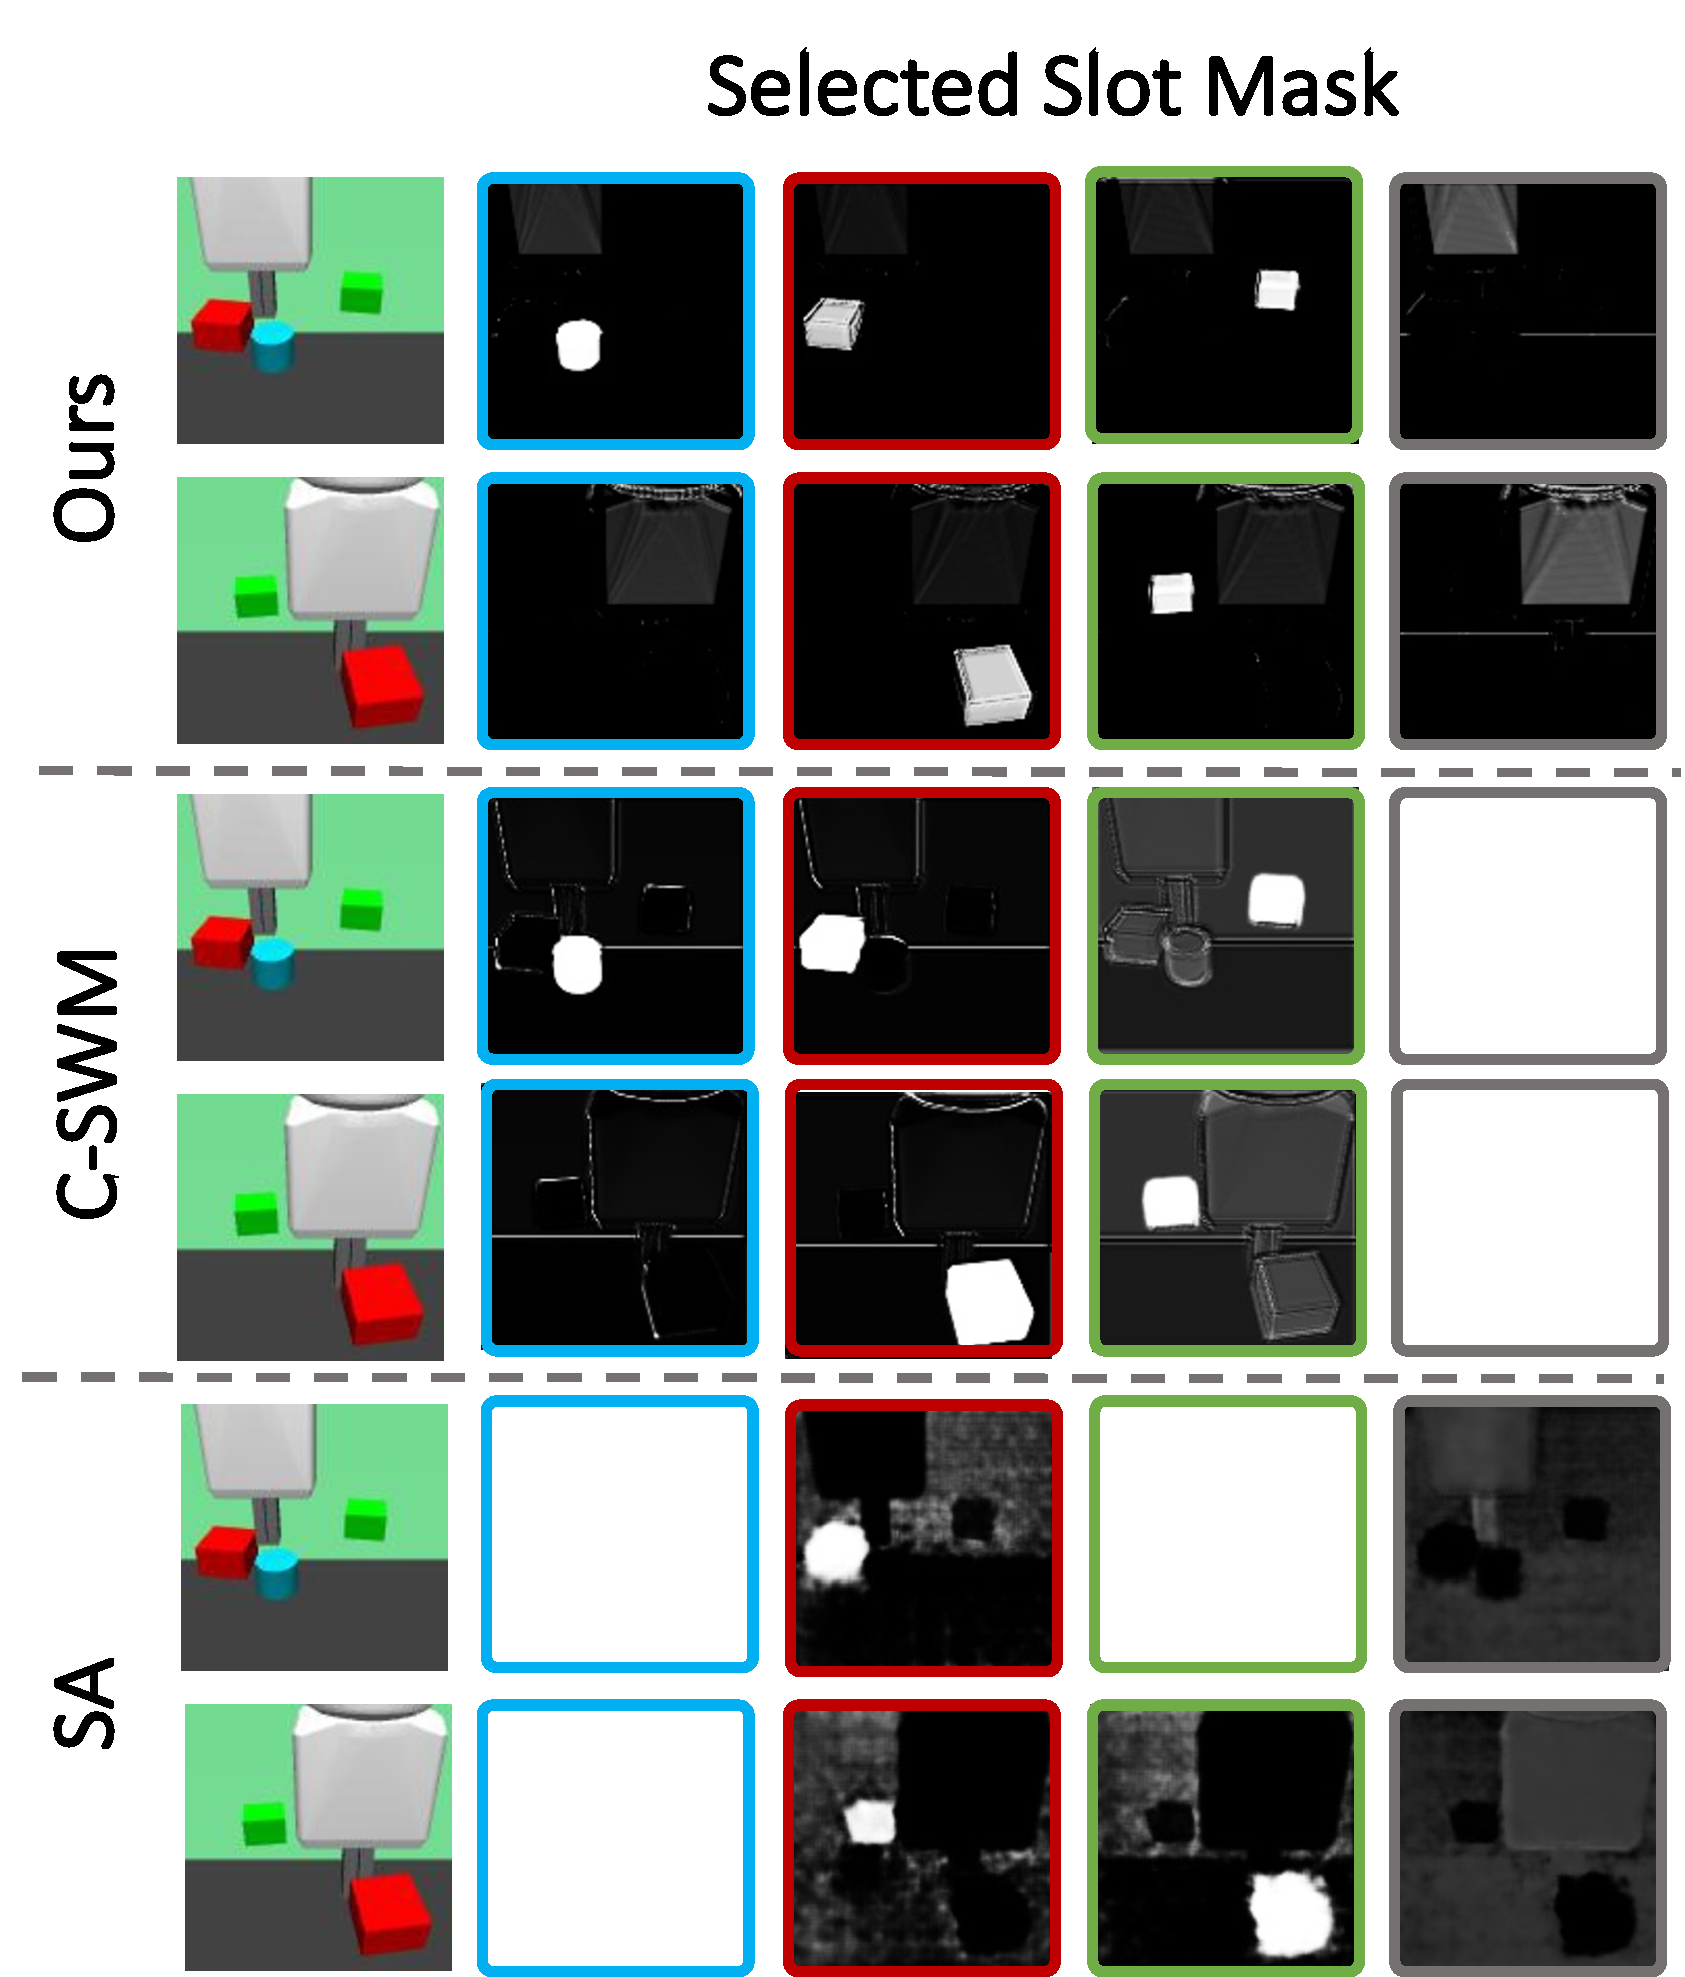
\includegraphics[height=0.3\textheight]{figs/qual_sim.pdf}
%  \caption{Examples of masks produced by \textsc{flood} and baselines on SIM images.}
%   \label{fig:qual_sim}
% \end{figure}
% \begin{figure}
%   \centering
  \caption{Examples of masks produced by \textsc{flood} and baselines on CUBES and SIM images. While C-SWM produces very crisp masks for all objects on CUBES, it interestingly fails to represent the robot (``object 4'') in SIM, despite the object-specific actions being easiest to specify for the robot. }
  \label{fig:qual_sim}
\end{figure}

\begin{figure}
  \centering
  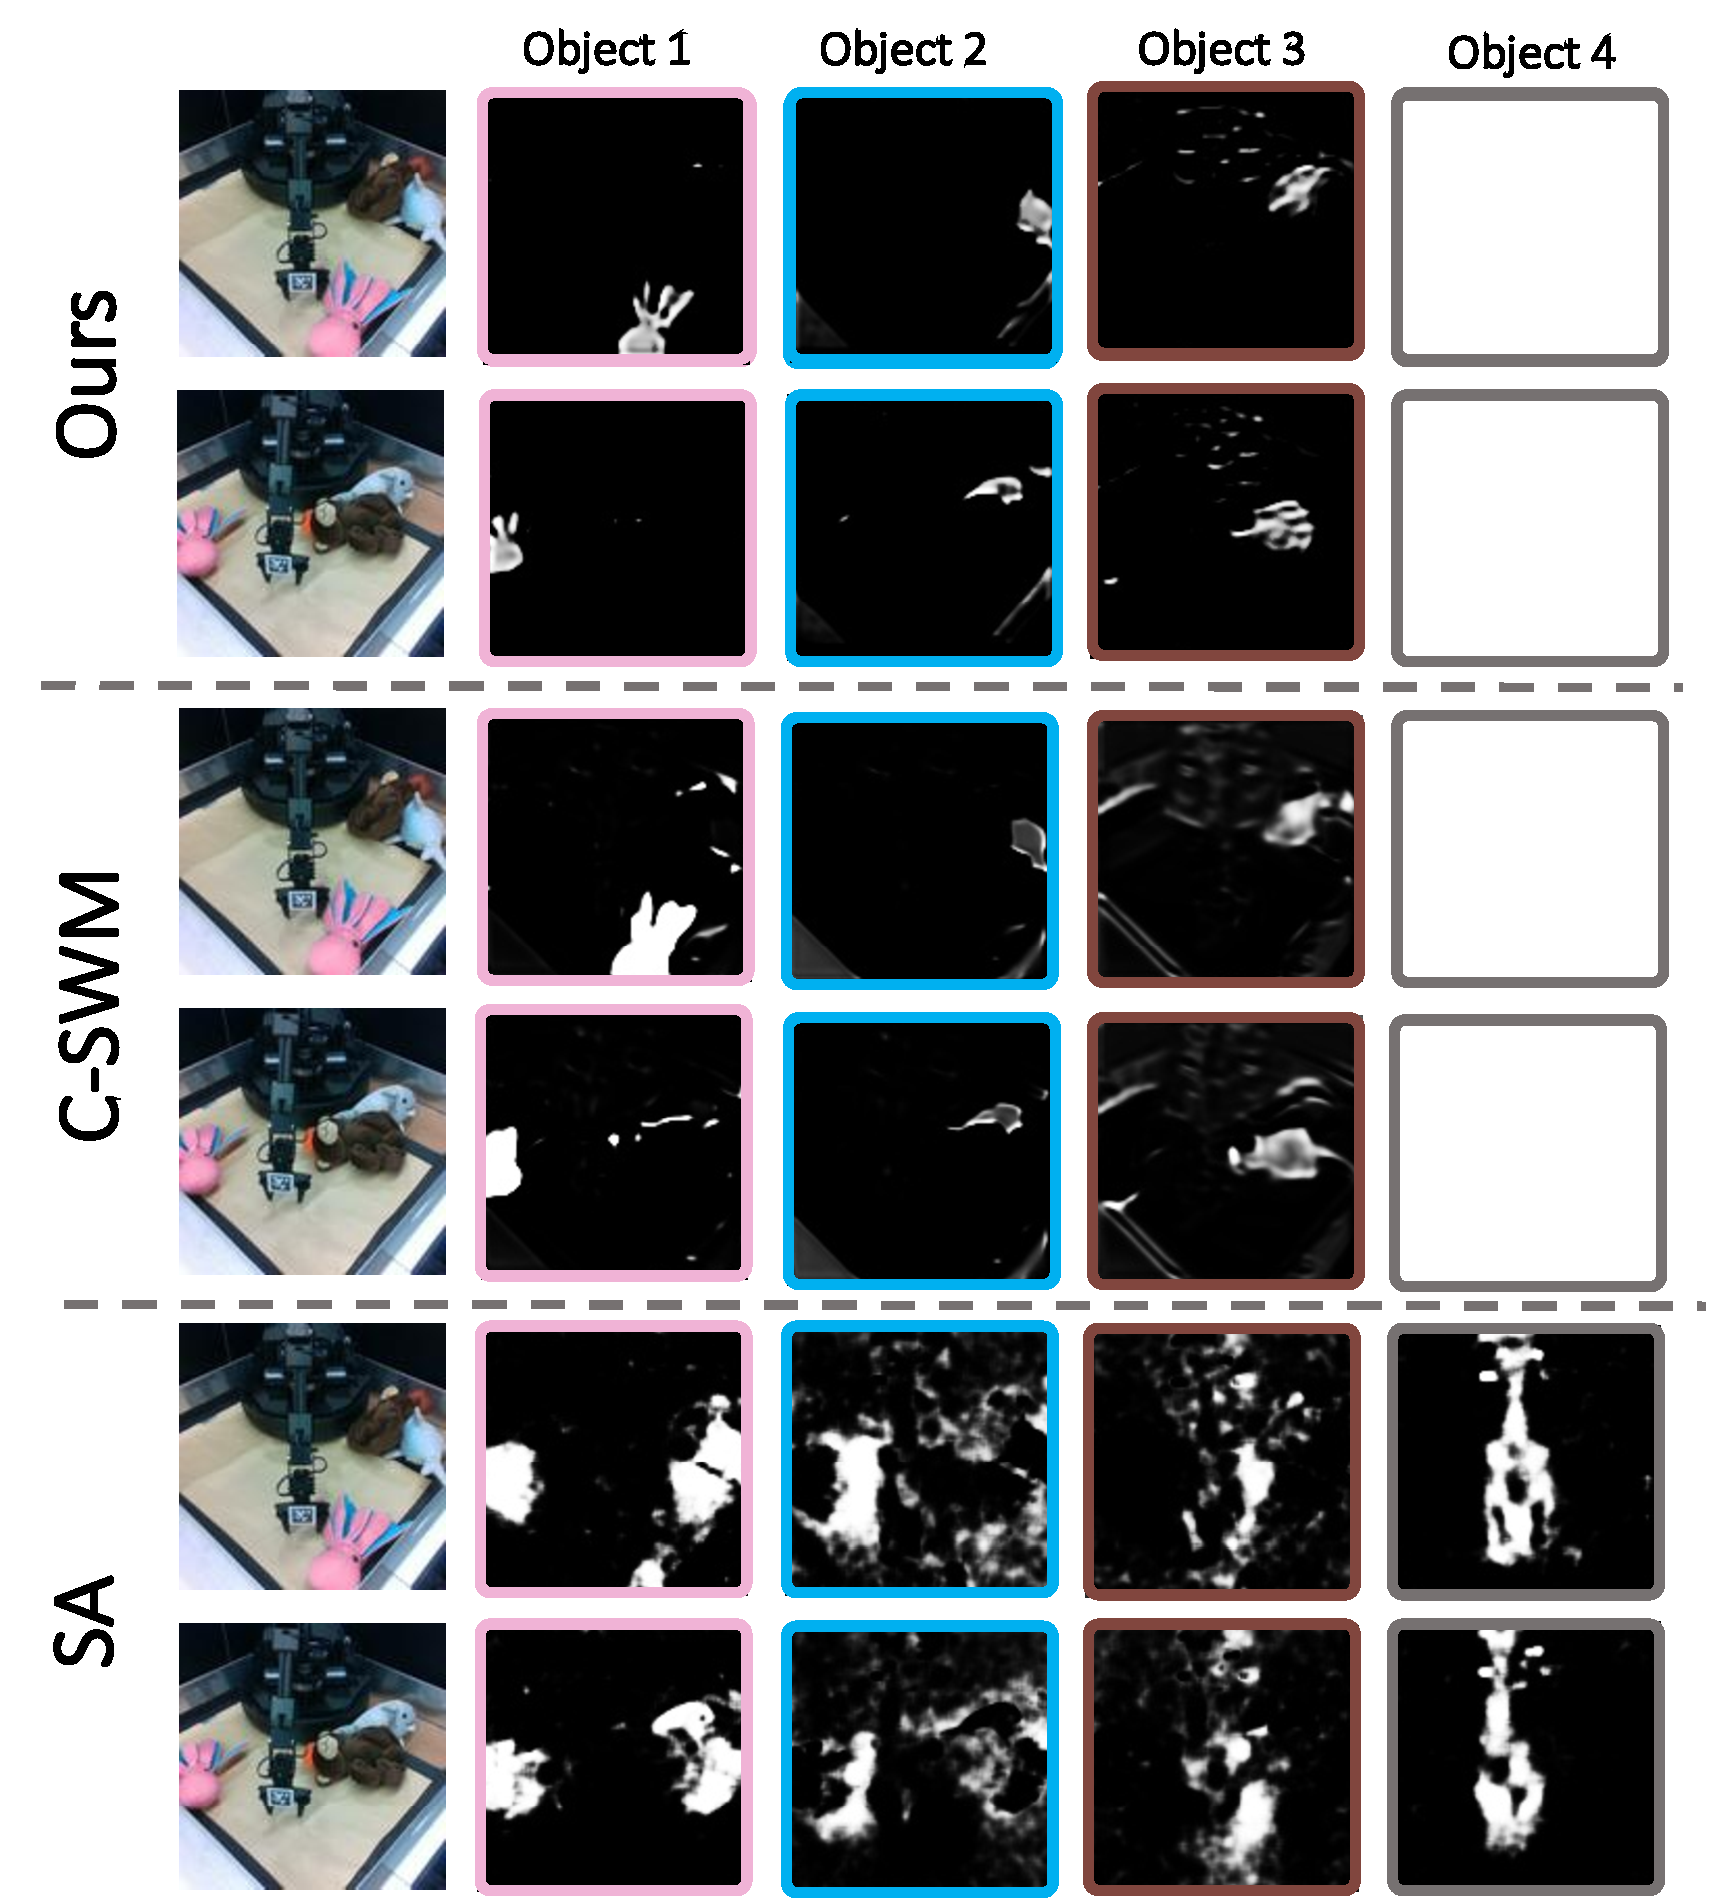
\includegraphics[height=0.45\textheight]{figs/qual_real.pdf}
  \caption{Examples of masks produced by \textsc{flood} and baselines on REAL images. This is the hardest setting, and all methods produce less crisp masks. However, C-SWM and our approach can both successfully learn to represent the three objects in the image, and both are unable to learn the robot.}
  \label{fig:qual_real}
\end{figure}


% \textbf{Question 1.} Does our method learn more accurate object centric representations?
% Metrics: 1) Slot Accuracy 

% \textbf{Question 2.} Does our method learn more disnentangled object-centric representations? Metrics: Slot compactness

% \textbf{Question 3.} Robustness to the number of slots?

%\jd{Prepare figures showing 1-2 nice examples for each dataset, perhaps a set of rows, where each row contains the input image, then the output masks of all baselines and our method for that image, similar to visualizations in papers like IODINE.}

%\subsection{Ablation}
%We show results for a controlled comparison of object discovery approaches in Table~\ref{table:objective}. For this experiment, we fix the object discovery network structure, and only change the training objective. In addition to the training objective used in our method, we adopted three other objectives: "dynamics modeling", "temporal continuity" and "reconstruction" from our baseline methods. Our training objective performs the best in terms of ARI, illustrating that our training objective produces the best quality slot masks comparing to all the other three baselines.
% \begin{itemize}
%     \item same C-SWM architecture: compare our flow-guided contrastive objective to C-SWM's objective (already there), SCN's temporal continuity objective, and standard reconstruction objective.
%     \item Qualitative analysis / failure examples 
%     \item sample efficiency
%     \item \#slots v.s. performance
%     \item what happens when we have k slots, n > k objects in the dataset, but only m < k objects in each image?
%     \item different ways to sample positive and negative
% \end{itemize}





\begin{comment}
\begin{table}
  \caption{Main evaluation results for slot representation quality. Best performance in \textbf{bold}}
  \label{sample-table}
  \centering
  \begin{tabular}{lllll}
    \toprule
    \multicolumn{1}{c}{} & \multicolumn{4}{c}{Real Control} \\
    \cmidrule(r){2-5}  
      & \textsc{flood}(Ours)      & C-SWM    & SCN     & SA  \\
    \cmidrule(r){2-5}
   KLME$\downarrow$  &   &  786.482287   & 806.727197&      \\
   \midrule
    ARI$\uparrow$     & 0.1685787  &  0.1596932  & - &   \\
    \bottomrule
  \end{tabular}
\end{table}

\begin{table}
  \caption{Sample table title}
  \label{sample-table}
  \centering
  \begin{tabular}{lllll}
    \toprule
    \multicolumn{1}{c}{} & \multicolumn{4}{c}{3D Blocks} \\
    \cmidrule(r){2-5}  
      & \textsc{flood}(Ours)      & C-SWM    & SCN     & SA  \\
    \midrule
   KLME$\downarrow$  &   &     & &      \\
   \midrule
    ARI$\uparrow$     &    &     & - &   \\
    \bottomrule
  \end{tabular}
\end{table}

\begin{comment}
\begin{table}
  \caption{Sample table title}
  \label{sample-table}
  \centering
  \begin{tabular}{lllll}
    \toprule
    \multicolumn{1}{c}{} & \multicolumn{4}{c}{3D Blocks} \\
    \cmidrule(r){2-5}  
      & KLME     & Slot Compactness     & Slot Modularity     & ARI  \\
    \midrule
    (Ours) &   &  &  &     \\
    C-SWM &    & &  &     \\
    Slot Contrastive &        & \\
    Slot Attention &    \\
    \bottomrule
  \end{tabular}
\end{table}
\begin{table}
  \caption{Sample table title}
  \label{sample-table}
  \centering
  \begin{tabular}{lllll}
    \toprule
    \multicolumn{1}{c}{} & \multicolumn{4}{c}{Simulated Control} \\
    \cmidrule(r){2-5}  
      & KLME$\downarrow$      & Slot Compactness$\uparrow$     & Slot Modularity$\uparrow$     & ARI$\uparrow$  \\
    \midrule
    (Ours) final s4 & 94.455135 &  0.38635144  & 0.0359788&0.41344     \\
    C-SWM not final &  &  0.45987  & 0.1717  &0.23062    \\
    Slot Contrastive final s4& 187.362204     & 0.098727525       & 0.05369954 & -\\
    Slot Attention &    \\
    \bottomrule
  \end{tabular}
\end{table}

\begin{table}
  \caption{Sample table title}
  \label{sample-table}
  \centering
  \begin{tabular}{lllll}
    \toprule
    \multicolumn{1}{c}{} & \multicolumn{4}{c}{Real Control} \\
    \cmidrule(r){2-5}  
      & KLME$\downarrow$     & Slot Compactness$\uparrow$     & Slot Modularity$\uparrow$      & ARI$\uparrow$   \\
    \midrule
    (Ours) &  & & &    0.1685787 \\
    C-SWM &       &   &&  0.1596932    \\
    Slot Contrastive final s4 & 555.432067285/9.4475     &    0.11556364/0.1131474 &0.08461118/0.067329510 & - \\ 
    Slot Attention &  & &   \\
    \bottomrule
  \end{tabular}
\end{table}
\end{comment}

\begin{table}
  \caption{Quantitative comparison of flow-guided (ours) vs. other training objectives on \textbf{SIM}}
  \label{table:objective}
  \resizebox{\textwidth}{!}{
  \centering
  \begin{tabular}{llllll}
    \toprule
    \multirow{3}{*}{\rotatebox[origin=c]{90}{\textbf{SIM}}} & & \textbf{\textsc{flood}(Ours)}      & \textbf{dynamics modeling}    & \textbf{temporal continuity}     & \textbf{reconstruction}  \\
    \cmidrule(r){2-6}
     & \textbf{ARI(\%)$\uparrow$}     &  \textbf{93.56}  & 70.93  & 7.89 & 33.35   \\
    \cmidrule(r){2-6}
    &  \textbf{KLME$\downarrow$}  & \textbf{100.86} &  \textbf{99.61}  & 455.04 & 396.82    \\
    %\midrule
    \bottomrule
  \end{tabular}
  }
\end{table}

\section{Conclusions}\label{sec:conclusions}

In this paper, we design a new approach for unsupervised object discovery that is informed by optical flow correspondences between neighboring images in video. We show that this easily outperforms baselines that learn object-structured representations from general videos, and even performs comparably with an approach that learns from additional object-specific information.

However, our approach is dependent on optical flow providing reliable correspondences. While optical flow approaches are mature, there remain difficulties in producing reliable correspondences in the presence of clutter, occlusions, and lighting changes. We do not handle such noisy correspondences in our approach, and leave it for future work. Our own experimental settings did not prove to suffer from these issues, but they may arise in still more challenging settings.

%these are still challenging tasks with more 


% \section{Citations, figures, tables, references}
% \label{others}

% These instructions apply to everyone.

% \subsection{Citations within the text}

% The \verb+natbib+ package will be loaded for you by default.  Citations may be
% author/year or numeric, as long as you maintain internal consistency.  As to the
% format of the references themselves, any style is acceptable as long as it is
% used consistently.

% The documentation for \verb+natbib+ may be found at
% \begin{center}
%   \url{http://mirrors.ctan.org/macros/latex/contrib/natbib/natnotes.pdf}
% \end{center}
% Of note is the command \verb+\citet+, which produces citations appropriate for
% use in inline text.  For example,
% \begin{verbatim}
%   \citet{hasselmo} investigated\dots
% \end{verbatim}
% produces
% \begin{quote}
%   Hasselmo, et al.\ (1995) investigated\dots
% \end{quote}

% If you wish to load the \verb+natbib+ package with options, you may add the
% following before loading the \verb+neurips_2021+ package:
% \begin{verbatim}
%   \PassOptionsToPackage{options}{natbib}
% \end{verbatim}

% If \verb+natbib+ clashes with another package you load, you can add the optional
% argument \verb+nonatbib+ when loading the style file:
% \begin{verbatim}
%   \usepackage[nonatbib]{neurips_2021}
% \end{verbatim}

% As submission is double blind, refer to your own published work in the third
% person. That is, use ``In the previous work of Jones et al.\ [4],'' not ``In our
% previous work [4].'' If you cite your other papers that are not widely available
% (e.g., a journal paper under review), use anonymous author names in the
% citation, e.g., an author of the form ``A.\ Anonymous.''

% \subsection{Footnotes}

% Footnotes should be used sparingly.  If you do require a footnote, indicate
% footnotes with a number\footnote{Sample of the first footnote.} in the
% text. Place the footnotes at the bottom of the page on which they appear.
% Precede the footnote with a horizontal rule of 2~inches (12~picas).

% Note that footnotes are properly typeset \emph{after} punctuation
% marks.\footnote{As in this example.}

% \subsection{Figures}

% \begin{figure}
%   \centering
%   \fbox{\rule[-.5cm]{0cm}{4cm} \rule[-.5cm]{4cm}{0cm}}
%   \caption{Sample figure caption.}
% \end{figure}

% All artwork must be neat, clean, and legible. Lines should be dark enough for
% purposes of reproduction. The figure number and caption always appear after the
% figure. Place one line space before the figure caption and one line space after
% the figure. The figure caption should be lower case (except for first word and
% proper nouns); figures are numbered consecutively.

% You may use color figures.  However, it is best for the figure captions and the
% paper body to be legible if the paper is printed in either black/white or in
% color.

% \subsection{Tables}

% All tables must be centered, neat, clean and legible.  The table number and
% title always appear before the table.  See Table~\ref{sample-table}.

% Place one line space before the table title, one line space after the
% table title, and one line space after the table. The table title must
% be lower case (except for first word and proper nouns); tables are
% numbered consecutively.

% Note that publication-quality tables \emph{do not contain vertical rules.} We
% strongly suggest the use of the \verb+booktabs+ package, which allows for
% typesetting high-quality, professional tables:
% \begin{center}
%   \url{https://www.ctan.org/pkg/booktabs}
% \end{center}
% This package was used to typeset Table~\ref{sample-table}.

% \begin{table}
%   \caption{Sample table title}
%   \label{sample-table}
%   \centering
%   \begin{tabular}{lll}
%     \toprule
%     \multicolumn{2}{c}{Part}                   \\
%     \cmidrule(r){1-2}
%     Name     & Description     & Size ($\mu$m) \\
%     \midrule
%     Dendrite & Input terminal  & $\sim$100     \\
%     Axon     & Output terminal & $\sim$10      \\
%     Soma     & Cell body       & up to $10^6$  \\
%     \bottomrule
%   \end{tabular}
% \end{table}

% \section{Final instructions}

% Do not change any aspects of the formatting parameters in the style files.  In
% particular, do not modify the width or length of the rectangle the text should
% fit into, and do not change font sizes (except perhaps in the
% \textbf{References} section; see below). Please note that pages should be
% numbered.

% \section{Preparing PDF files}

% Please prepare submission files with paper size ``US Letter,'' and not, for
% example, ``A4.''

% Fonts were the main cause of problems in the past years. Your PDF file must only
% contain Type 1 or Embedded TrueType fonts. Here are a few instructions to
% achieve this.

% \begin{itemize}

% \item You should directly generate PDF files using \verb+pdflatex+.

% \item You can check which fonts a PDF files uses.  In Acrobat Reader, select the
%   menu Files$>$Document Properties$>$Fonts and select Show All Fonts. You can
%   also use the program \verb+pdffonts+ which comes with \verb+xpdf+ and is
%   available out-of-the-box on most Linux machines.

% \item The IEEE has recommendations for generating PDF files whose fonts are also
%   acceptable for NeurIPS. Please see
%   \url{http://www.emfield.org/icuwb2010/downloads/IEEE-PDF-SpecV32.pdf}

% \item \verb+xfig+ "patterned" shapes are implemented with bitmap fonts.  Use
%   "solid" shapes instead.

% \item The \verb+\bbold+ package almost always uses bitmap fonts.  You should use
%   the equivalent AMS Fonts:
% \begin{verbatim}
%   \usepackage{amsfonts}
% \end{verbatim}
% followed by, e.g., \verb+\mathbb{R}+, \verb+\mathbb{N}+, or \verb+\mathbb{C}+
% for $\mathbb{R}$, $\mathbb{N}$ or $\mathbb{C}$.  You can also use the following
% workaround for reals, natural and complex:
% \begin{verbatim}
%   \newcommand{\RR}{I\!\!R} %real numbers
%   \newcommand{\Nat}{I\!\!N} %natural numbers
%   \newcommand{\CC}{I\!\!\!\!C} %complex numbers
% \end{verbatim}
% Note that \verb+amsfonts+ is automatically loaded by the \verb+amssymb+ package.

% \end{itemize}

% If your file contains type 3 fonts or non embedded TrueType fonts, we will ask
% you to fix it.

% \subsection{Margins in \LaTeX{}}

% Most of the margin problems come from figures positioned by hand using
% \verb+\special+ or other commands. We suggest using the command
% \verb+\includegraphics+ from the \verb+graphicx+ package. Always specify the
% figure width as a multiple of the line width as in the example below:
% \begin{verbatim}
%   \usepackage[pdftex]{graphicx} ...
%   \includegraphics[width=0.8\linewidth]{myfile.pdf}
% \end{verbatim}
% See Section 4.4 in the graphics bundle documentation
% (\url{http://mirrors.ctan.org/macros/latex/required/graphics/grfguide.pdf})

% A number of width problems arise when \LaTeX{} cannot properly hyphenate a
% line. Please give LaTeX hyphenation hints using the \verb+\-+ command when
% necessary.

% \begin{ack}
% Use unnumbered first level headings for the acknowledgments. All acknowledgments
% go at the end of the paper before the list of references. Moreover, you are required to declare
% funding (financial activities supporting the submitted work) and competing interests (related financial activities outside the submitted work).
% More information about this disclosure can be found at: \url{https://neurips.cc/Conferences/2021/PaperInformation/FundingDisclosure}.

% Do {\bf not} include this section in the anonymized submission, only in the final paper. You can use the \texttt{ack} environment provided in the style file to autmoatically hide this section in the anonymized submission.
% \end{ack}

% \section*{References}

% References follow the acknowledgments. Use unnumbered first-level heading for
% the references. Any choice of citation style is acceptable as long as you are
% consistent. It is permissible to reduce the font size to \verb+small+ (9 point)
% when listing the references.
% Note that the Reference section does not count towards the page limit.
% \medskip

\bibliography{refs}

%%%%%%%%%%%%%%%%%%%%%%%%%%%%%%%%%%%%%%%%%%%%%%%%%%%%%%%%%%%%
\section*{Checklist}

%%% BEGIN INSTRUCTIONS %%%
The checklist follows the references.  Please
read the checklist guidelines carefully for information on how to answer these
questions.  For each question, change the default \answerTODO{} to \answerYes{},
\answerNo{}, or \answerNA{}.  You are strongly encouraged to include a {\bf
justification to your answer}, either by referencing the appropriate section of
your paper or providing a brief inline description.  For example:
\begin{itemize}
  \item Did you include the license to the code and datasets? \answerYes{See Section~\ref{gen_inst}.}
  \item Did you include the license to the code and datasets? \answerNo{The code and the data are proprietary.}
  \item Did you include the license to the code and datasets? \answerNA{}
\end{itemize}
Please do not modify the questions and only use the provided macros for your
answers.  Note that the Checklist section does not count towards the page
limit.  In your paper, please delete this instructions block and only keep the
Checklist section heading above along with the questions/answers below.
%%% END INSTRUCTIONS %%%

\begin{enumerate}

\item For all authors...
\begin{enumerate}
  \item Do the main claims made in the abstract and introduction accurately reflect the paper's contributions and scope?
    \answerYes{See abstract}
  \item Did you describe the limitations of your work?
    \answerYes{we discussed the limiations of our method in conclusion. We will include additional analysis of limitations of our work in supplemental material}
  \item Did you discuss any potential negative societal impacts of your work?
    \answerNo{We do not focus on specific applications in this work. Like any such basic research approaches, while applications might have the potential for negative impacts, it is difficult to meaningfully foresee them for this work.}
  \item Have you read the ethics review guidelines and ensured that your paper conforms to them?
    \answerYes{}
\end{enumerate}

\item If you are including theoretical results...
\begin{enumerate}
  \item Did you state the full set of assumptions of all theoretical results?
    \answerNA{}
	\item Did you include complete proofs of all theoretical results?
    \answerNA{}
\end{enumerate}

\item If you ran experiments...
\begin{enumerate}
  \item Did you include the code, data, and instructions needed to reproduce the main experimental results (either in the supplemental material or as a URL)?
    \answerYes{We cited the works that we took our dataset from. We will include our code and dataset in the supplemental material}
  \item Did you specify all the training details (e.g., data splits, hyperparameters, how they were chosen)?
    \answerYes{In section 3.4 and 4.2}
	\item Did you report error bars (e.g., with respect to the random seed after running experiments multiple times)?
    \answerNA{}
	\item Did you include the total amount of compute and the type of resources used (e.g., type of GPUs, internal cluster, or cloud provider)?
    \answerYes{In section 3.4}
\end{enumerate}

\item If you are using existing assets (e.g., code, data, models) or curating/releasing new assets...
\begin{enumerate}
  \item If your work uses existing assets, did you cite the creators?
    \answerYes{In section 4.2}
  \item Did you mention the license of the assets?
    \answerYes{We cite the paper that we took the dataset from in section 4.2}
  \item Did you include any new assets either in the supplemental material or as a URL?
    \answerNo{}
  \item Did you discuss whether and how consent was obtained from people whose data you're using/curating?
    \answerYes{}
  \item Did you discuss whether the data you are using/curating contains personally identifiable information or offensive content?
    \answerYes{No they don't contain personally identifiable information or offensive content.}
\end{enumerate}

\item If you used crowdsourcing or conducted research with human subjects...
\begin{enumerate}
  \item Did you include the full text of instructions given to participants and screenshots, if applicable?
    \answerNA{}
  \item Did you describe any potential participant risks, with links to Institutional Review Board (IRB) approvals, if applicable?
    \answerNA{}
  \item Did you include the estimated hourly wage paid to participants and the total amount spent on participant compensation?
    \answerNA{}
\end{enumerate}

\end{enumerate}

%%%%%%%%%%%%%%%%%%%%%%%%%%%%%%%%%%%%%%%%%%%%%%%%%%%%%%%%%%%%

\end{document}